%Compile with XeLatex
\documentclass[11pt]{scrartcl} % Font size


%----------------------------------------------------------------------------------------
%	PACKAGES AND OTHER DOCUMENT CONFIGURATIONS
%----------------------------------------------------------------------------------------

\usepackage{amsmath, amsfonts, amsthm} % Math packages

\usepackage{listings} % Code listings, with syntax highlighting
\lstset{ 
	language=Matlab, % choose the language of the code
%	basicstyle=10pt, % the size of the fonts that are used for the code
	numbers=left,    % where to put the line-numbers
	numberstyle=\footnotesize,% the size of the fonts that are used for the line-numbers
	stepnumber=1,% the step between two line-numbers. If it's 1 each line will be numbered
	numbersep=5pt,% how far the line-numbers are from the code
%	backgroundcolor=\color{white},  	% choose the background color. You must add \usepackage{color}
	showspaces=false, % show spaces adding particular underscores
	showstringspaces=false,% underline spaces within strings
	showtabs=false,% show tabs within strings adding particular underscores
%	frame=single,	% adds a frame around the code
%	tabsize=2, 		% sets default tabsize to 2 spaces
%	captionpos=b, 			% sets the caption-position to bottom
	breaklines=true,   			% sets automatic line breaking
	breakatwhitespace=false, % sets if automatic breaks should only happen at whitespace
	escapeinside={\%*}{*)} % if you want to add a comment within your code
}
\usepackage{fontspec,xgreek,polyglossia}

\usepackage{hyperref}
\setdefaultlanguage{greek}
\setotherlanguage[]{english} % Greek (main) and English language hyphenation
\setmainfont{Times New Roman}
\setsansfont{Arial}
\setmonofont{DejaVu Sans Mono}
\newfontfamily\greekfont[Script=Greek]{Linux Libertine O}
\newfontfamily\greekfontsf[Script=Greek]{Linux Libertine O}
\usepackage{graphicx} % Required for inserting images
\usepackage{float}
\graphicspath{{Figures/}{./}} % Specifies where to look for included images (trailing slash required)

\usepackage{booktabs} % Required for better horizontal rules in tables

\numberwithin{equation}{section} % Number equations within sections (i.e. 1.1, 1.2, 2.1, 2.2 instead of 1, 2, 3, 4)
\numberwithin{figure}{section} % Number figures within sections (i.e. 1.1, 1.2, 2.1, 2.2 instead of 1, 2, 3, 4)
\numberwithin{table}{section} % Number tables within sections (i.e. 1.1, 1.2, 2.1, 2.2 instead of 1, 2, 3, 4)

\setlength\parindent{0pt} % Removes all indentation from paragraphs

\usepackage{enumitem} % Required for list customisation
\setlist{noitemsep} % No spacing between list items

%----------------------------------------------------------------------------------------
%	DOCUMENT MARGINS
%----------------------------------------------------------------------------------------

\usepackage{geometry} % Required for adjusting page dimensions and margins

\geometry{
	paper=a4paper, % Paper size, change to letterpaper for US letter size
	top=2.5cm, % Top margin
	bottom=3cm, % Bottom margin
	left=3cm, % Left margin
	right=3cm, % Right margin
	headheight=0.75cm, % Header height
	footskip=1.5cm, % Space from the bottom margin to the baseline of the footer
	headsep=0.75cm, % Space from the top margin to the baseline of the header
	%showframe, % Uncomment to show how the type block is set on the page
}

%----------------------------------------------------------------------------------------
%	FONTS
%----------------------------------------------------------------------------------------

\usepackage[utf8]{inputenc} % Required for inputting international characters
\usepackage[T1]{fontenc} % Use 8-bit encoding

\usepackage{fourier} % Use the Adobe Utopia font for the document

%----------------------------------------------------------------------------------------
%	SECTION TITLES
%----------------------------------------------------------------------------------------

\usepackage{sectsty} % Allows customising section commands

\sectionfont{\vspace{6pt}\centering\normalfont\scshape} % \section{} styling
\subsectionfont{\normalfont\bfseries} % \subsection{} styling
\subsubsectionfont{\normalfont\itshape} % \subsubsection{} styling
\paragraphfont{\normalfont\scshape} % \paragraph{} styling

%----------------------------------------------------------------------------------------
%	HEADERS AND FOOTERS
%----------------------------------------------------------------------------------------

\usepackage{scrlayer-scrpage} % Required for customising headers and footers

\ohead*{} % Right header
\ihead*{} % Left header
\chead*{} % Centre header

\ofoot*{} % Right footer
\ifoot*{} % Left footer
\cfoot*{\pagemark} % Centre footer
 % Include the file specifying the document structure and custom commands

\title{	
	\normalfont\normalsize
	\textsc{ Αριστοτέλειο Πανεπιστήμιο Θεσσαλονίκης, Σχολή Θετικών Επιστημών, Τμήμα Φυσικής}\\ % Your university, school and/or department name(s)
	\vspace{25pt} % Whitespace
	\rule{\linewidth}{0.5pt}\\ % Thin top horizontal rule
	\vspace{20pt} % Whitespace
	{\huge Εργασία στο Μάθημα Ανάλυση Δεδομένων }\\ % The assignment title
	\vspace{12pt} % Whitespace
	\rule{\linewidth}{2pt}\\ % Thick bottom horizontal rule
	\vspace{12pt} % Whitespace
}

\author{\LARGE Κίμων Ζαγκούρης \\ A.E.M. 4353 \\ Email: kzagko@gmail.com} % Your name

\date{\normalsize\today} % Today's date (\today) or a custom date

\begin{document}

\maketitle


\begin{figure}[H]
	\centering
	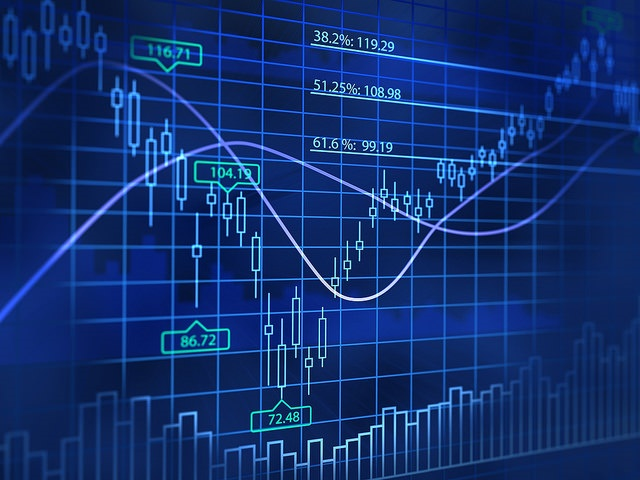
\includegraphics[width=0.7\columnwidth]{Main.jpg}
\end{figure}
\footnote{Image created by Timashov Sergiy.}
\newpage


\tableofcontents
\newpage



\section{Ζητήματα}
\label{sec:z}
Παρακάτω είναι τα 10 ζητήματα της εργασίας αυτής ανά κεφάλαιο. Στο \hyperref[sec:Prog]{Κεφάλαιο \ref*{sec:Prog}} υπάρχουν τα αντίστοιχα προγράμματα Matlab που χρησιμοποιήθηκαν για την επίλυση των ζητημάτων.


\subsection{Ζήτημα 1}
\label{subsec:z1}
Στο ζήτημα αυτό τρέχουμε τον παρακάτω \hyperref[mat:1]{Κώδικα} για 6 περιπτώσεις και παραθέτουμε τα γραφήματα.

\begin{figure}[H] 
\label{fig:1}
	\centering
	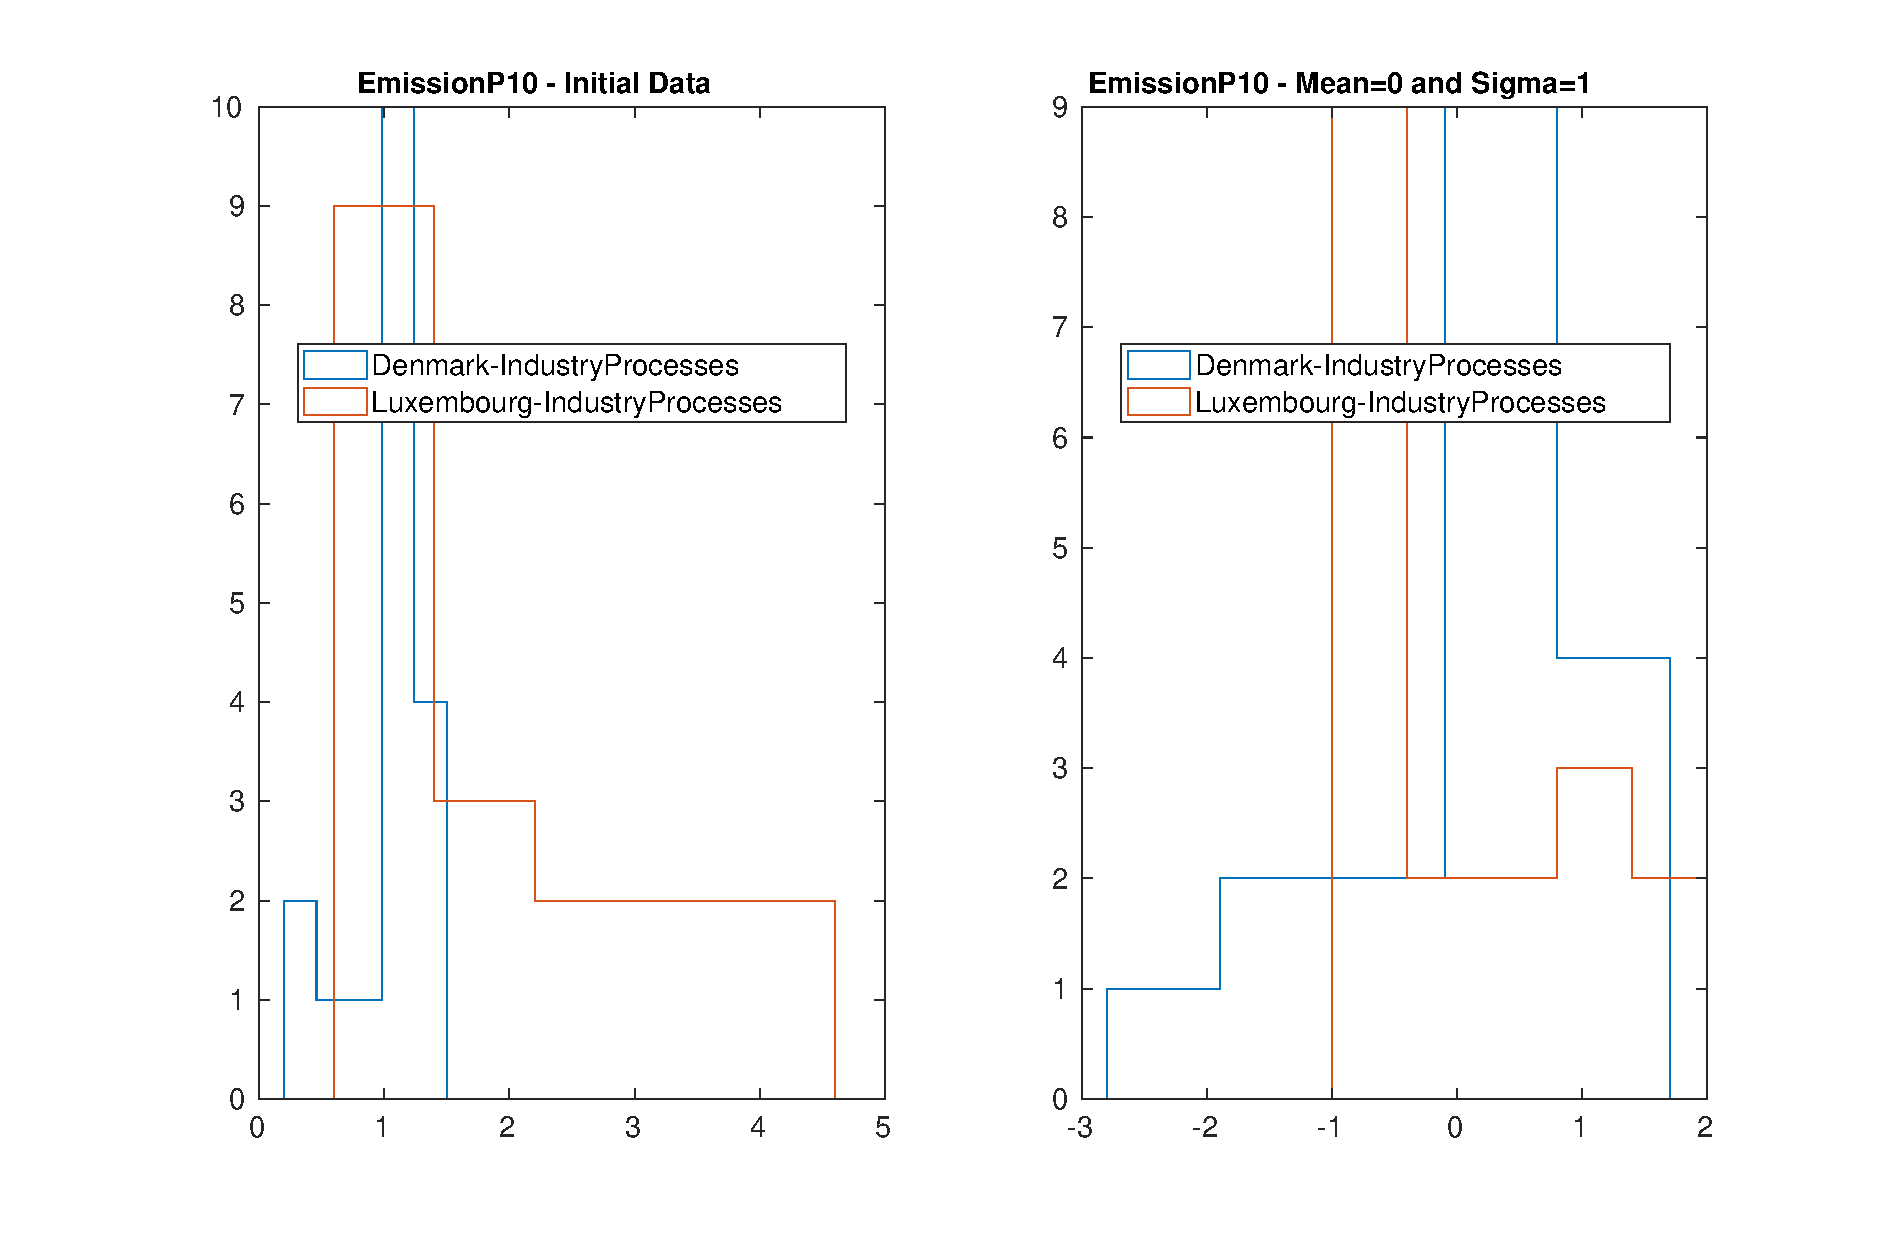
\includegraphics[width=1\columnwidth]{Ex1/Denmark_Luxembourg_IndustryProcesses_hist.eps}	
	\caption{PM10 Emissions for Denmark Luxembourg IndustryProcesses. }
\end{figure}

\begin{figure}[H] 
\label{fig:2}
	\centering
	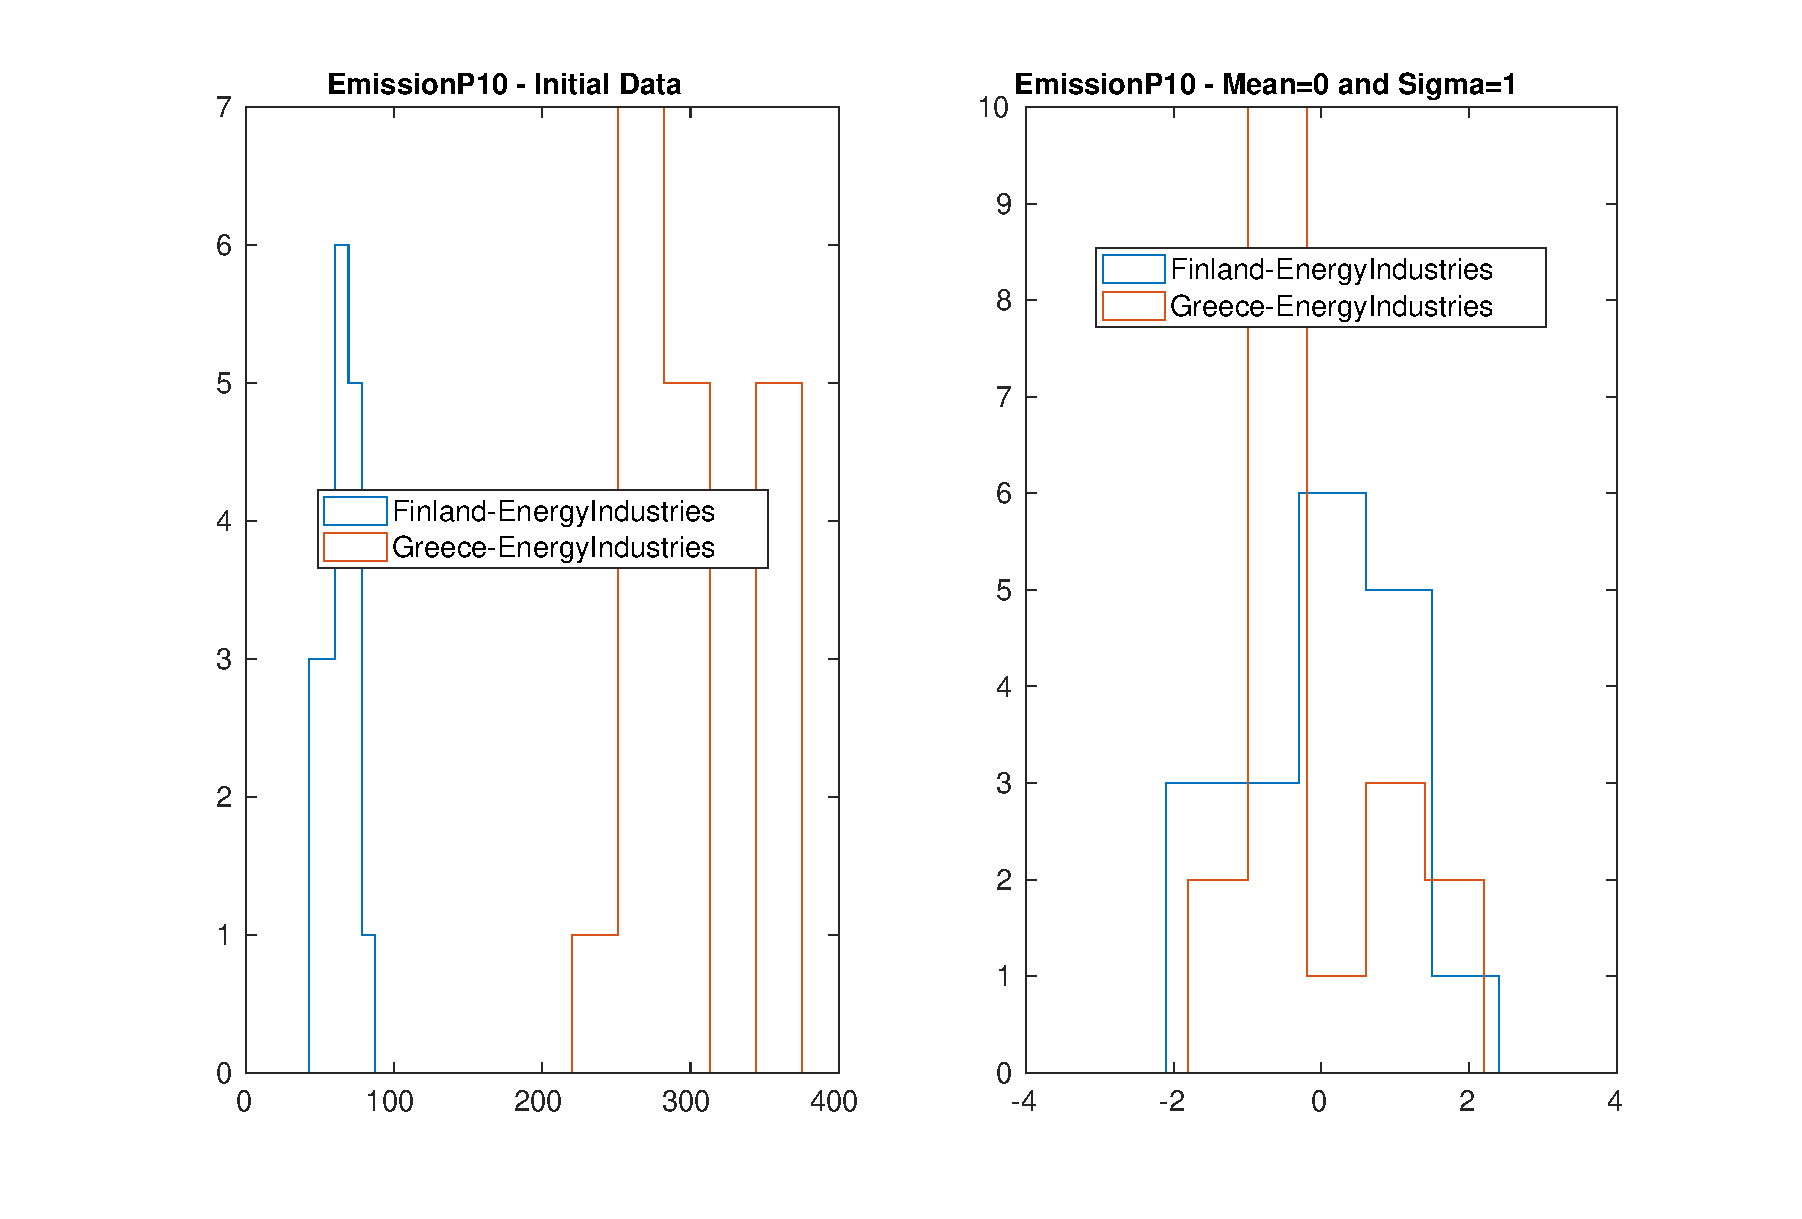
\includegraphics[width=1\columnwidth]{Ex1/Finland_Greece_EnergyIndustries_hist.eps}	
	\caption{PM10 Emissions for Finland Greece EnergyIndustries.}
\end{figure}

\begin{figure}[H] 
	\label{fig:3}
	\centering
	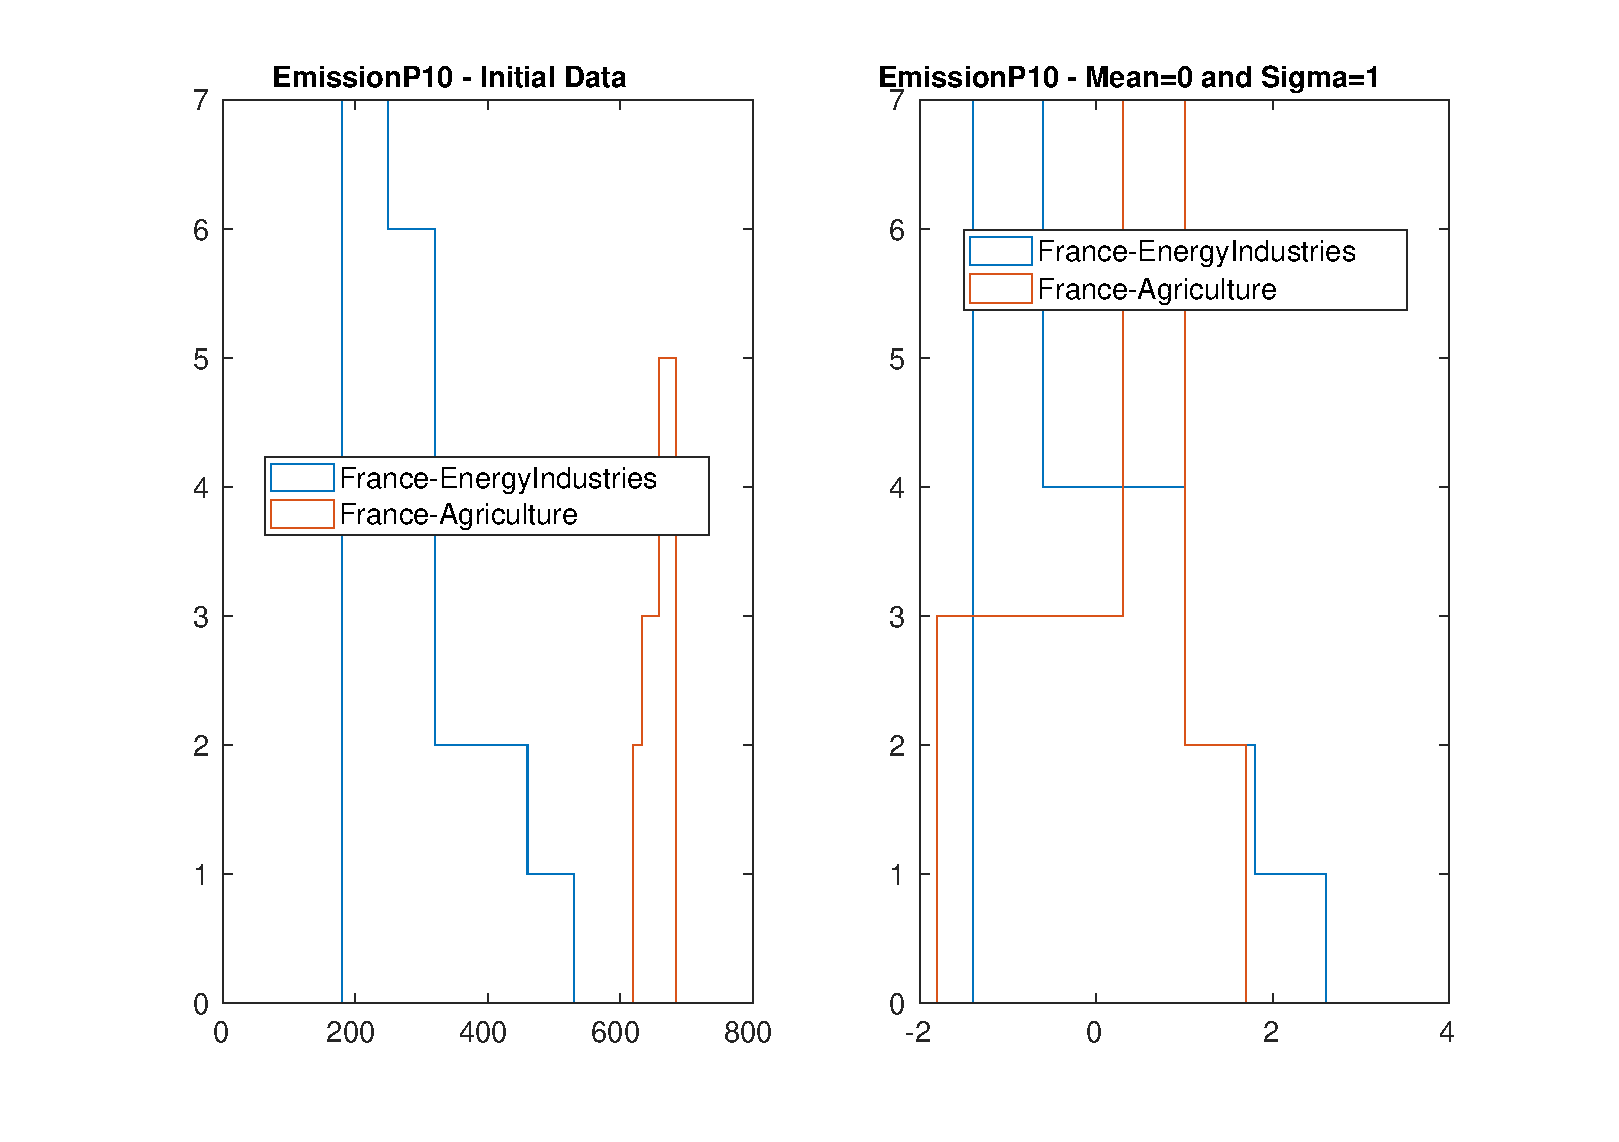
\includegraphics[width=1\columnwidth]{Ex1/France_EnergyIndustries_Agriculture_hist.eps}	
\caption{PM10 Emissions for France EnergyIndustries Agriculture.}
\end{figure}


\begin{figure}[H]
\label{fig:4} 
	\centering
	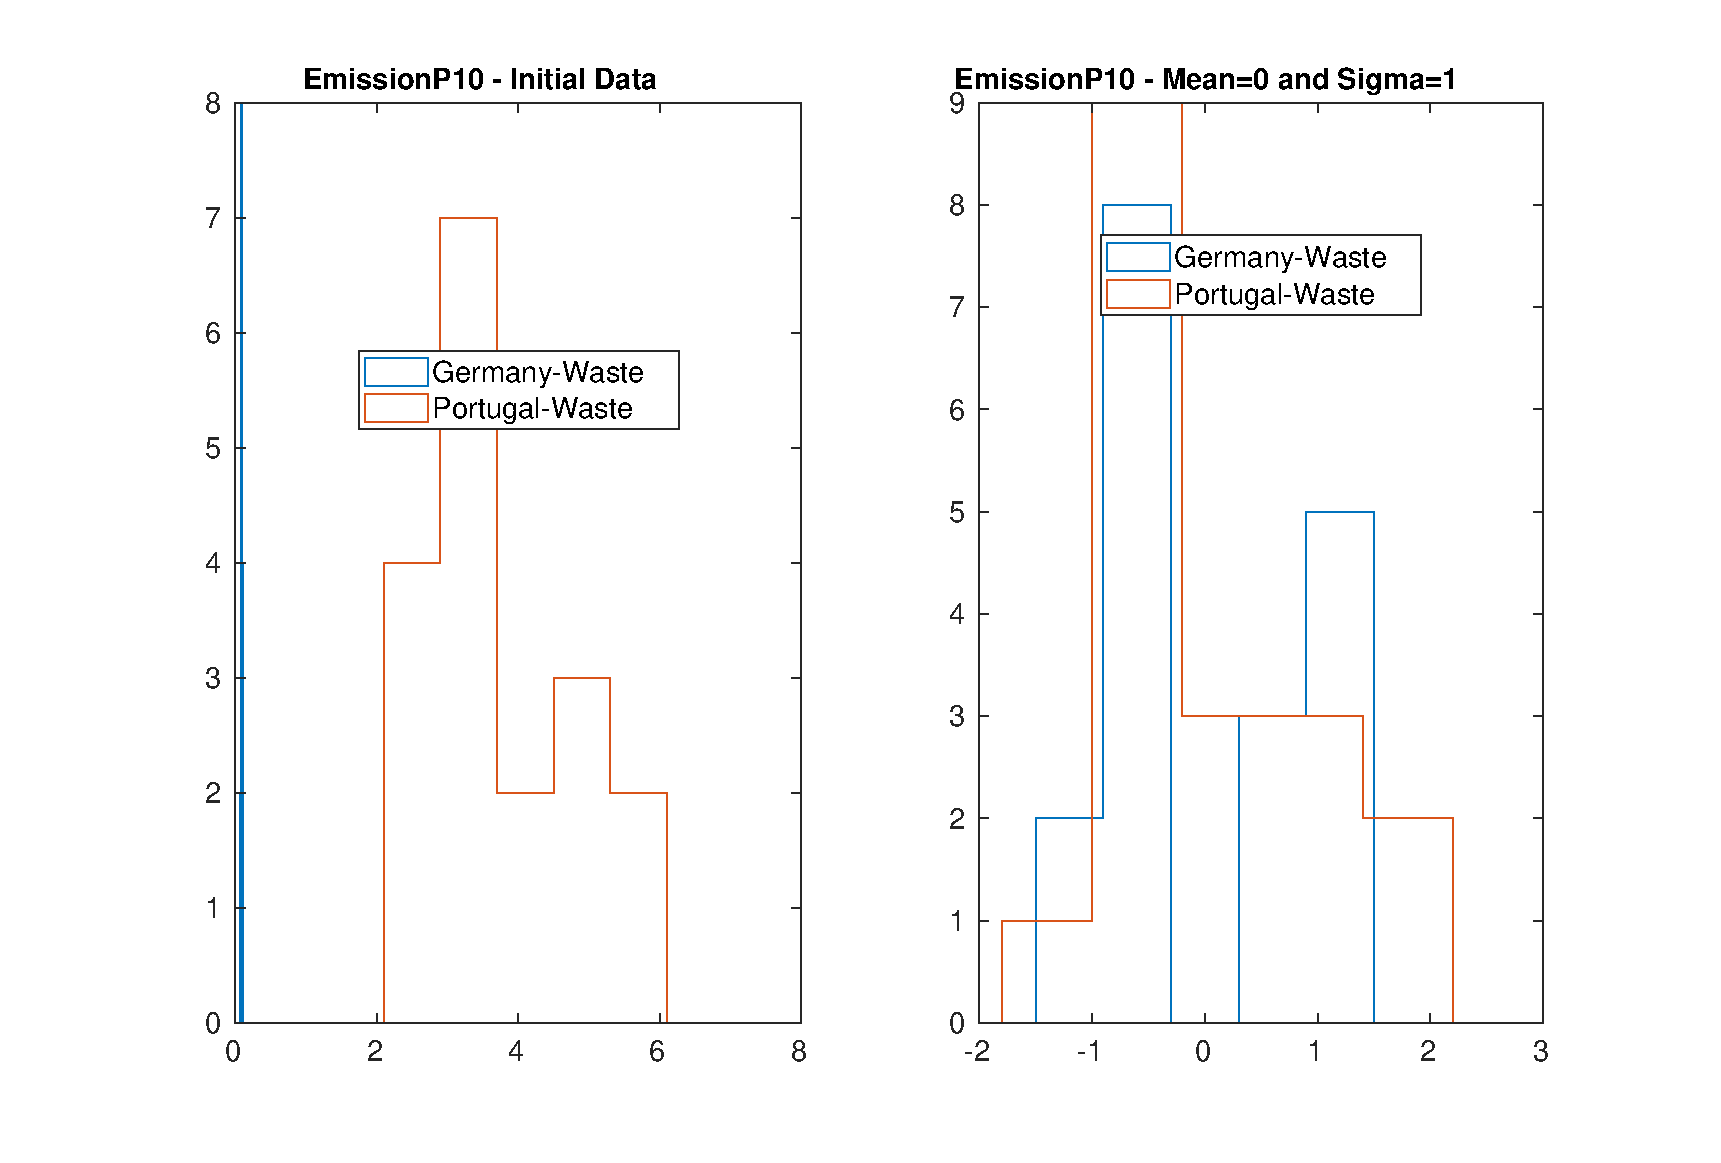
\includegraphics[width=1\columnwidth]{Ex1/Germany_Portugal_Waste_hist.eps}	
\caption{PM10 Emissions for Germany Portugal Waste.}
\end{figure}


\begin{figure}[H] 
	\label{fig:5}
	\centering
	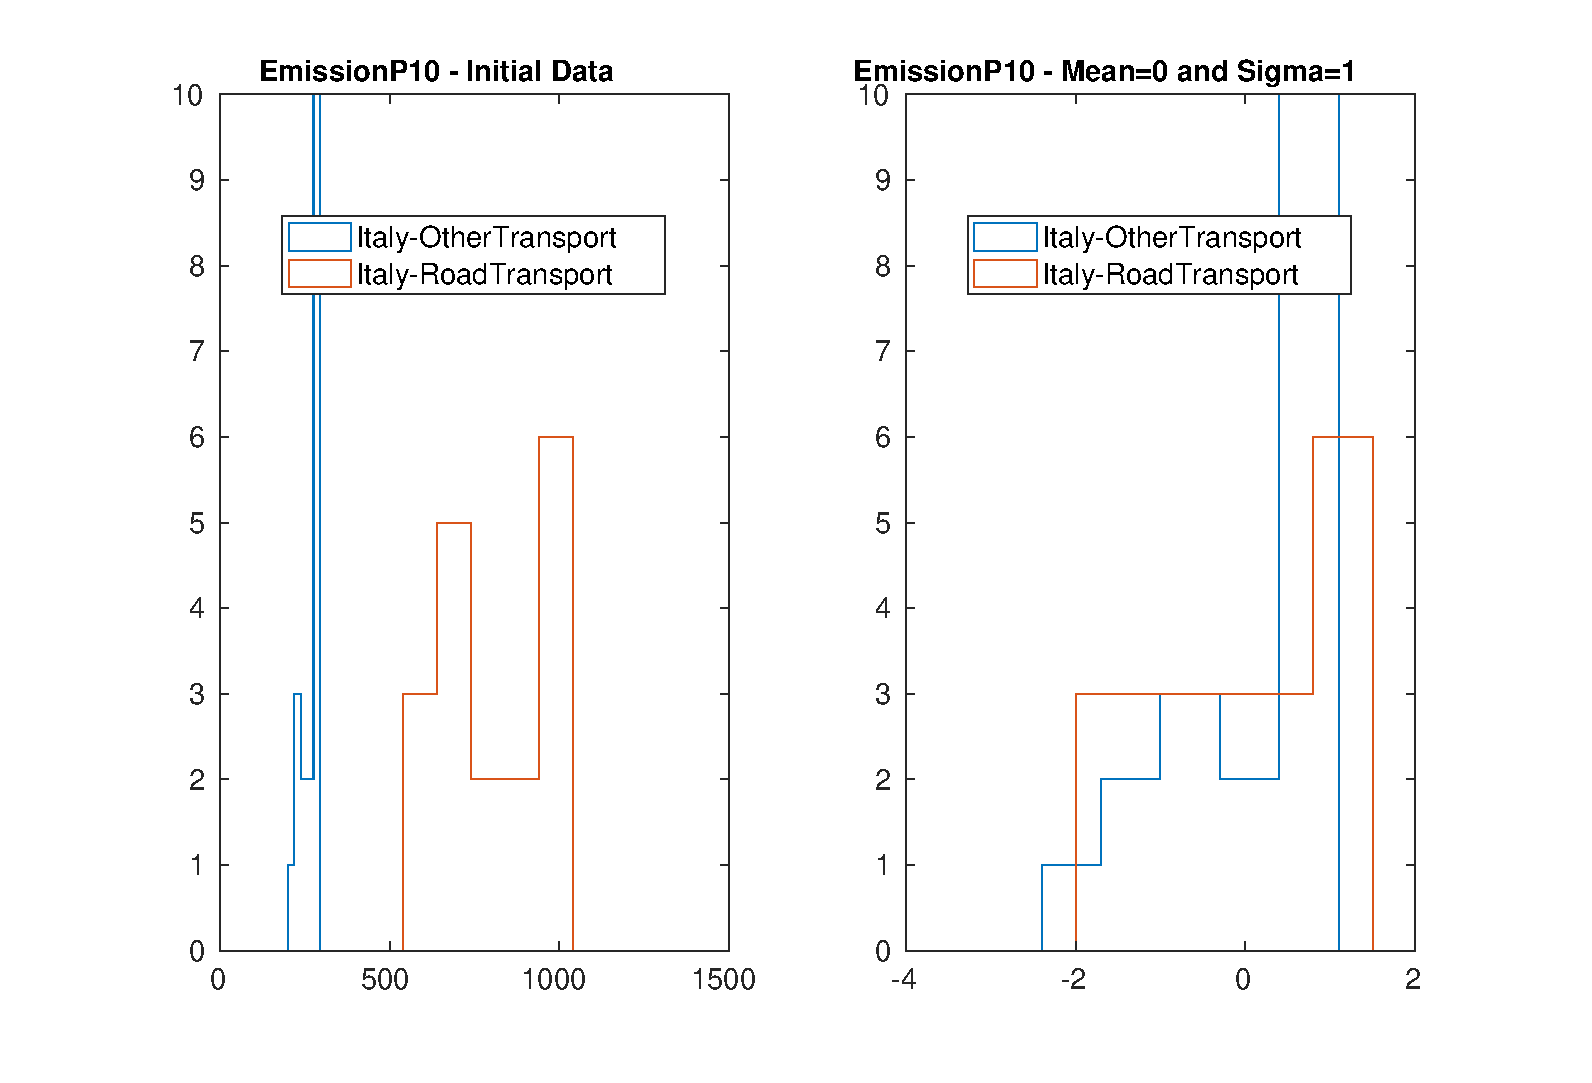
\includegraphics[width=1\columnwidth]{Ex1/Italy_OtherTransport_RoadTransport_hist.eps}	
	\caption{PM10 Emissions for Italy OtherTransport RoadTransport.}
\end{figure}

\begin{figure}[H]
\label{fig:6} 
	\centering
	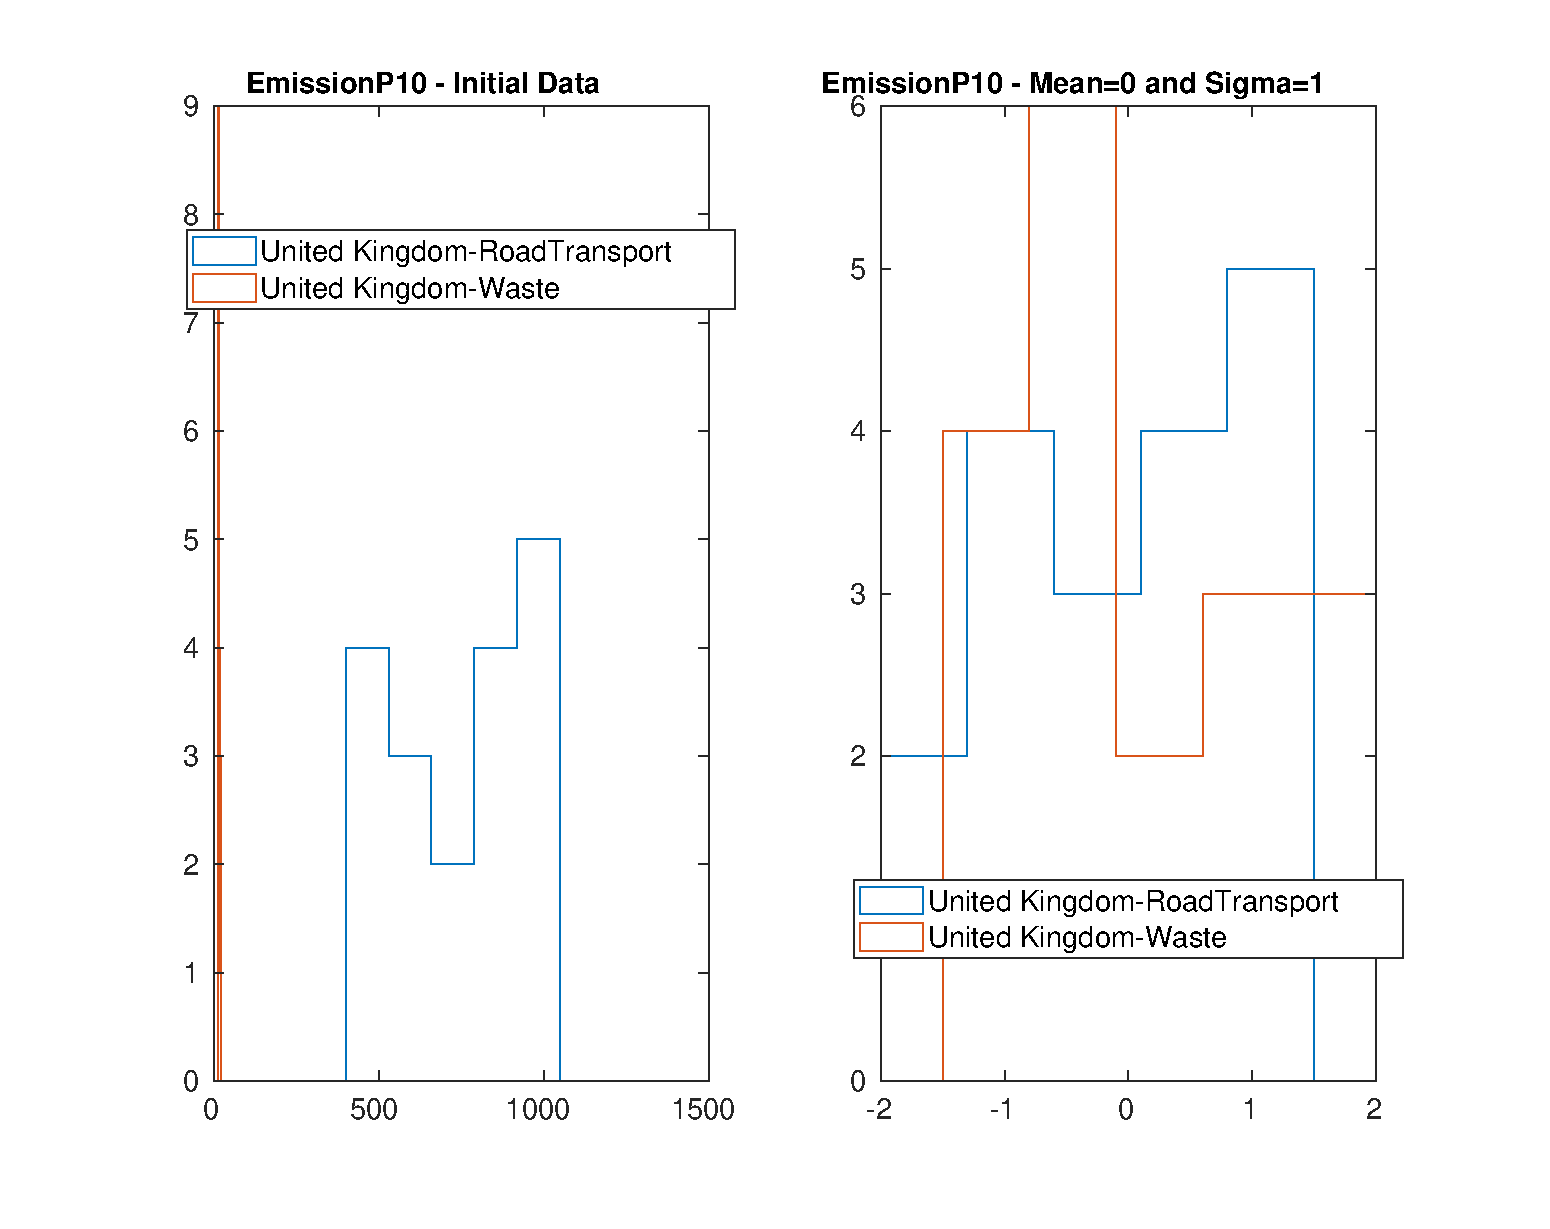
\includegraphics[width=1\columnwidth]{Ex1/United-Kingdom_RoadTransport_Waste_hist.eps}	
\caption{PM10 Emissions for United Kingdom RoadTransport Waste.}
\end{figure}


Τα παραπάνω αποτελούν ένα τυχαίο δείγμα από όλα τα δυνατά αποτελέσματα και συνδυασμούς των χωρών και των δραστηριοτήτων αλλά μπορούμε να σχολιάσουμε μερικά από αυτά. Στο \hyperref[fig:3]{σχήμα \ref*{fig:3}} βλέπουμε ότι οι κατανομές των PM10 πριν την κανονικοποίηση δεν είναι εύκολο να συγκριθούν και να ελεγχθούν αλλά μετά την κανονικοποίηση μπορούμε να πούμε ότι φαίνεται να μην έχουν κοινή κατανομή λόγω του σχήματός τους. Ενώ αντίθετα στο \hyperref[fig:5]{σχήμα \ref*{fig:5}} Για την κατανομή των PM10 στην Ιταλία βλέπουμε ότι όταν κανονικοποιούμε τις κατανομές φαίνεται αυτές να μοιάζουν. Γενικά όμως τα δεδομένα είναι λίγα, στην καλύτερη περίπτωση 18 σημεία, τα οποία όταν κατανέμονται σε ιστόγραμμα δίνουν πολύ μικρό αριθμό στοιχείων, περίπου 4, ανά περιοχή κατανομής (bin). Με αποτέλεσμα να είναι δύσκολο να έχουμε καλή περιγραφή της κάθε κατανομής. 

\subsection{Ζήτημα 2}
\label{subsec:z2}
Για την επίλυση αυτού του ζητήματος κάνουμε χρήση του \hyperref[mat:2]{κώδικα \ref*{mat:2}}. Λόγου του μικρού αριθμού δεδομένων η συνάρτηση chi2gof του Matlab δεν επιστρέφει αξιόπιστα αποτελέσματα για τον υπολογισμό του $\chi^{2}$. Για τον λόγο αυτό στο παραπάνω πρόγραμμα επιλέξαμε να κάνουμε αναλυτική μέτρηση του $\chi^{2}$. Μετά την εκτέλεση το πρόγραμμα μας επιστρέφει τα παρακάτω σχήματα \ref{fig:z21} και \ref{fig:z22}.



\begin{figure}[H]
\label{fig:z21} 
	\centering
	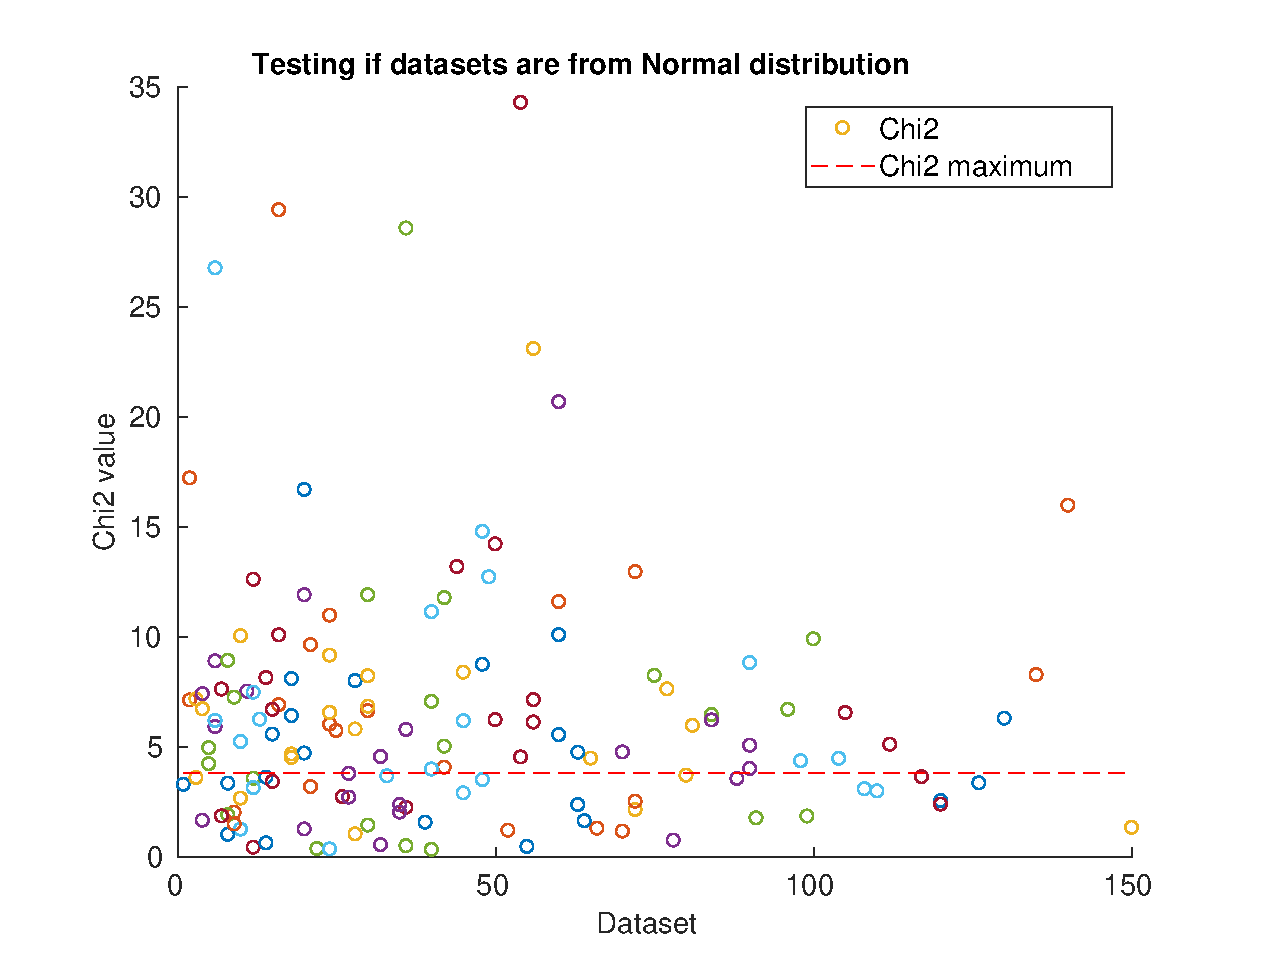
\includegraphics[width=1\columnwidth]{Ex2/ChiDistr.eps}	
\caption{Αποτελέσματα $\chi^{2}$ για κάθε δραστηριότητα και χώρα καθώς και το μέγιστο όριο με διακεκομμένη γραμμή.}
\end{figure}

Από το \hyperref[fig:z21]{σχήμα \ref*{fig:z21}} παρατηρούμε ότι αρκετά 
$\chi^{2}$ βρίσκονται επάνω από το μέγιστο $\chi^{2}_{1-\alpha,n-3}$. Για τους βαθμούς ελευθερίας χρησιμοποιούμε $n-3$ γιατί συγκρίνουμε με την συνεχή κανονική κατανομή που έχει δύο ακόμα δεσμευτικές παραμέτρους, την μέση τιμή και την απόκλιση.


Το πρόγραμμα επίσης μας επιστρέφει αν βρήκε μια κατανομή να είναι κανονική ή όχι με βάση κάποιο όριο πιθανότητας. Παρακάτω είναι τα αποτελέσματα αυτού του ελέγχου.

\begin{verbatim}
At the significance level of  5.00% the percentage of the datasets
that could be from a Normal distribution are 37.33% 

At the confindence level of  5.00%

Does Agriculture Follow a normal distribution : YES
Does EnergyIndustries Follow a normal distribution : YES
Does EnergyIndustriesPowerProduction1A1a Follow a normal distribution : NO
Does FugitiveEmissions Follow a normal distribution : NO
Does IndustryEnergy Follow a normal distribution : NO
Does IndustryProcesses Follow a normal distribution : YES
Does OtherEnergy Follow a normal distribution : YES
Does OtherTransport Follow a normal distribution : NO
Does RoadTransport Follow a normal distribution : NO
Does Waste Follow a normal distribution : NO
\end{verbatim}

Παρατηρούμε ότι στο επίπεδο σημαντικότητας $5\%$ περίπου το $37\%$ από όλα τα σετ θα μπορούσε να θεωρηθεί ότι προέρχεται από κανονική κατανομή. Επίσης στο ίδιο ποσοστό σημαντικότητας βλέπουμε ότι μόνο 4 στις 10 δραστηριότητες θα μπορούσαν να προέρχονται από κανονική κατανομή.

\begin{figure}[H]
\label{fig:z22} 
	\centering
	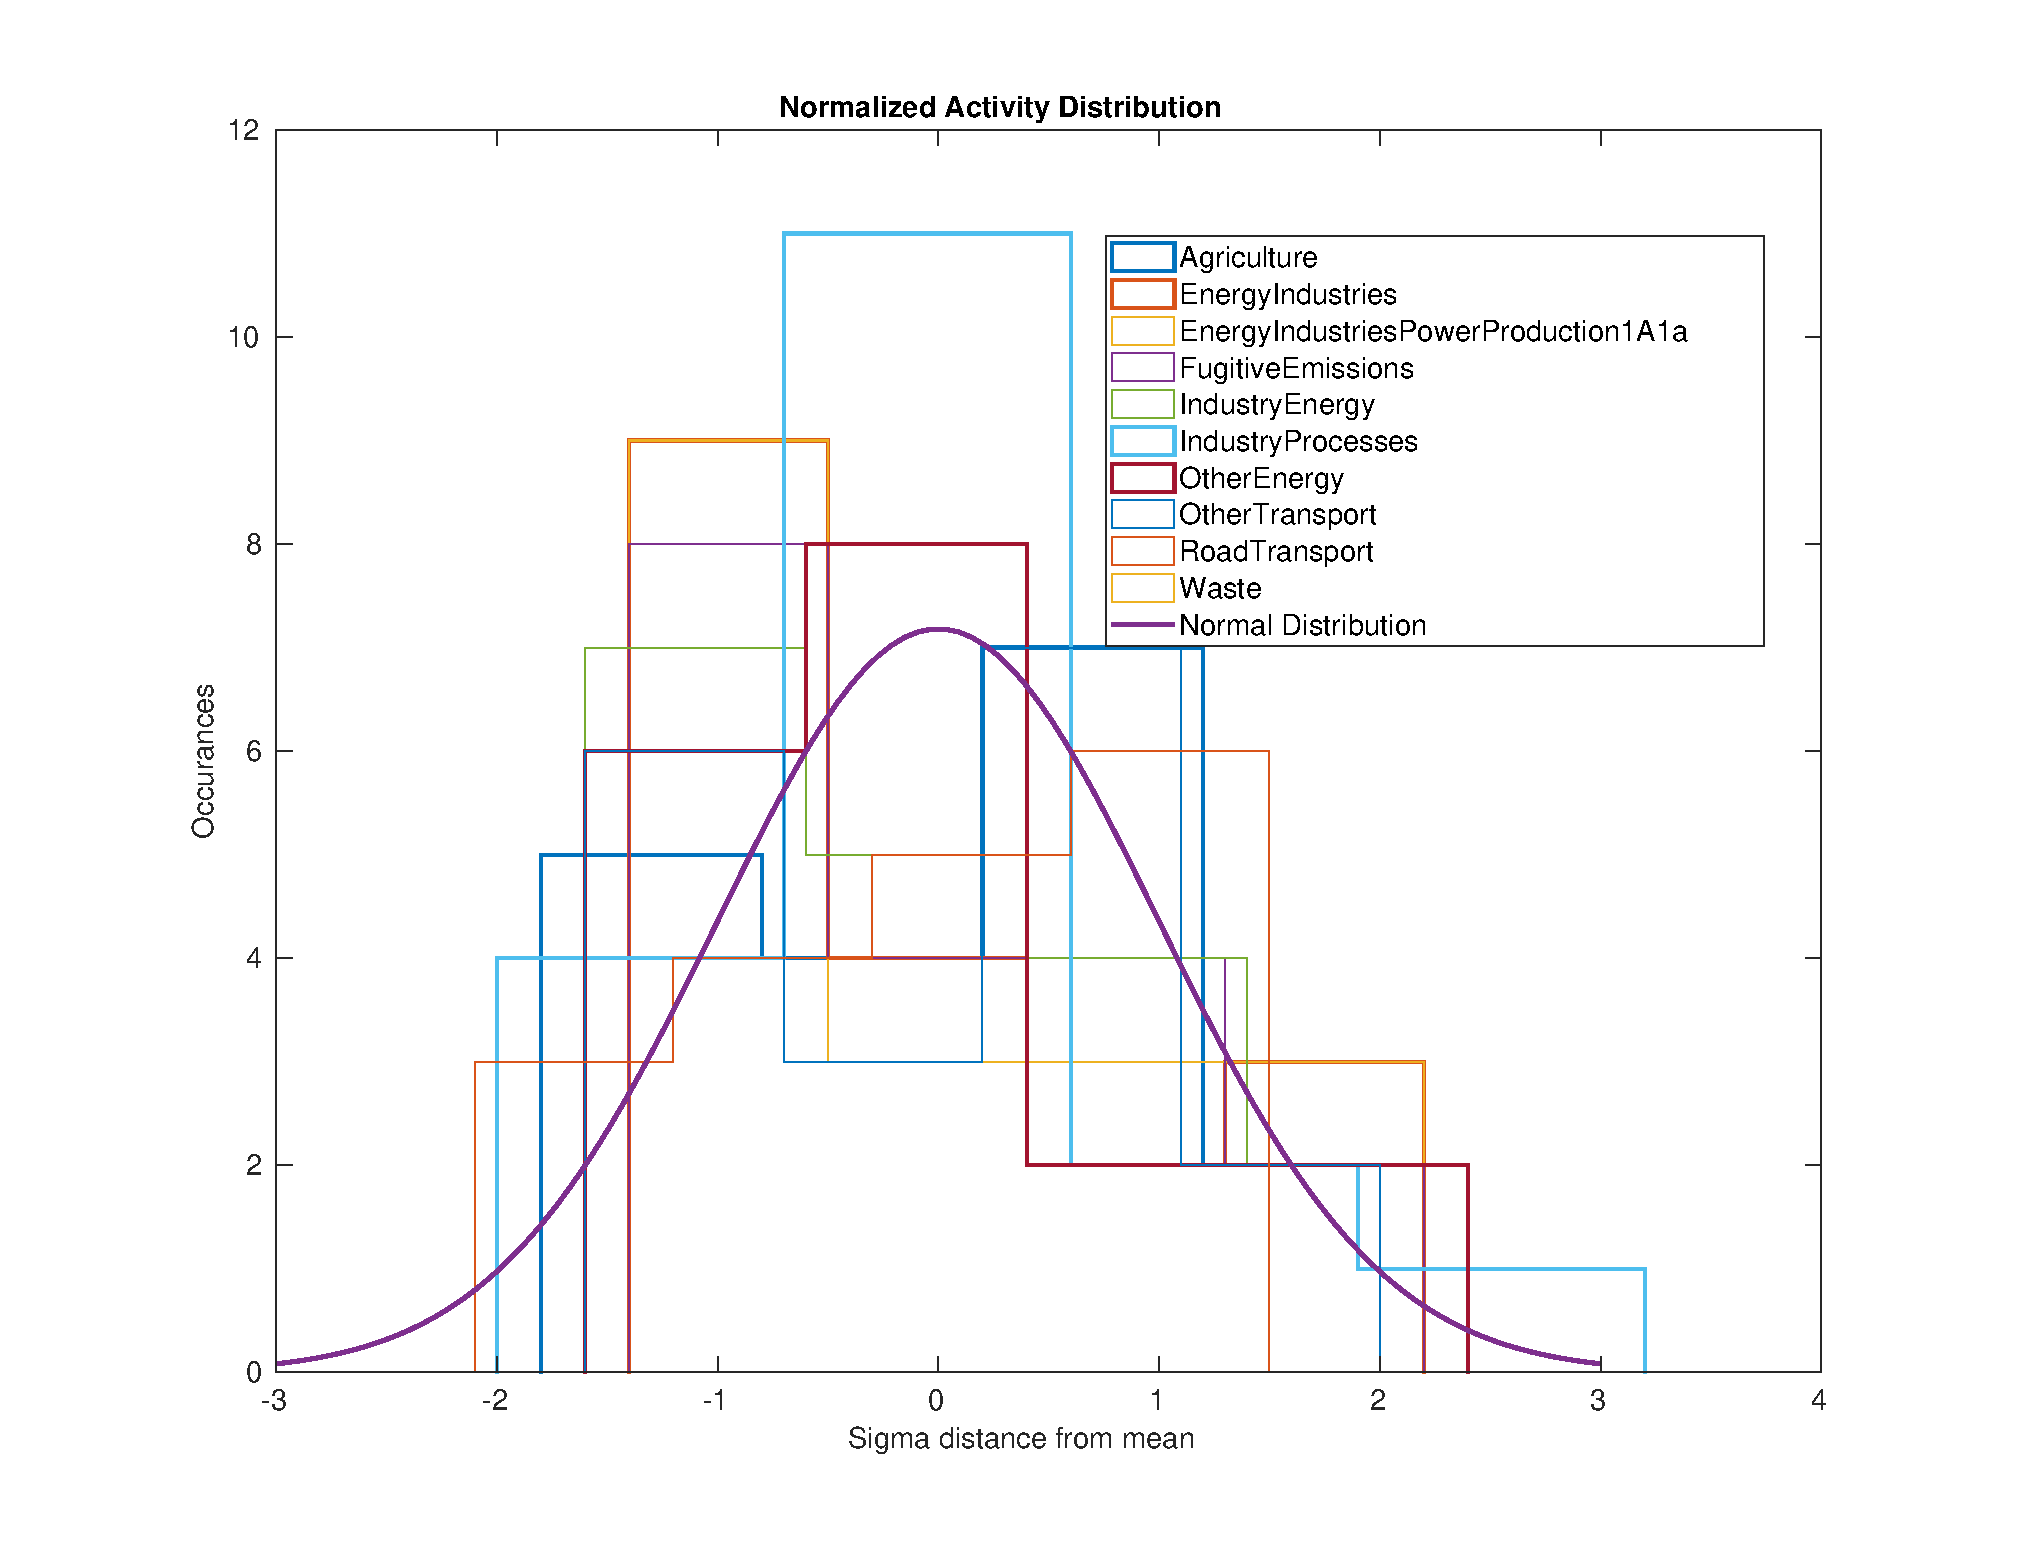
\includegraphics[width=1\columnwidth]{Ex2/ActDistr.eps}	
\caption{Κανονικοποιημένες συνολικές κατανομές για όλες τις δραστηριότητες καθώς και ενδεικτική κανονική κατανομή για σύγκριση. Οι δραστηριότητες με ποιο έντονη γραμμή έχουν περάσει το τεστ κανονικότητας.}
\end{figure}

Στο \hyperref[fig:z22]{σχήμα \ref*{fig:z22}} παρατηρούμε ότι γενικά οι κανονικοποιημένες κατανομές των δραστηριοτήτων διαφέρουν από κανονικές. Πέρα απο τα αποτελέσματα που μας επιστρέφει το πρόγραμμα θα μπορούσε κάποιος οπτικά και μόνο να πει ότι από όλες τις κατανομές αυτές που φαίνεται να ακολουθούν κανονική κατανομή είναι: IndustryProcesses και OtherEnergy.   






\subsection{Ζήτημα 3}
\label{subsec:z3}

Για την επίλυση αυτού του ζητήματος κάνουμε χρήση του \hyperref[mat:3]{κώδικα \ref*{mat:3}}. Ενδεικτικά εκτελέσαμε τον κώδικα για 4 δραστηριότητες και τα αποτελέσματα φαίνονται στα \hyperref[fig:z31]{σχήμα \ref*{fig:z31}},\hyperref[fig:z32]{σχήμα \ref*{fig:z32}},\hyperref[fig:z33]{σχήμα \ref*{fig:z33}} και \hyperref[fig:z34]{σχήμα \ref*{fig:z34}}.


\begin{figure}[H]
\label{fig:z31} 
	\centering
	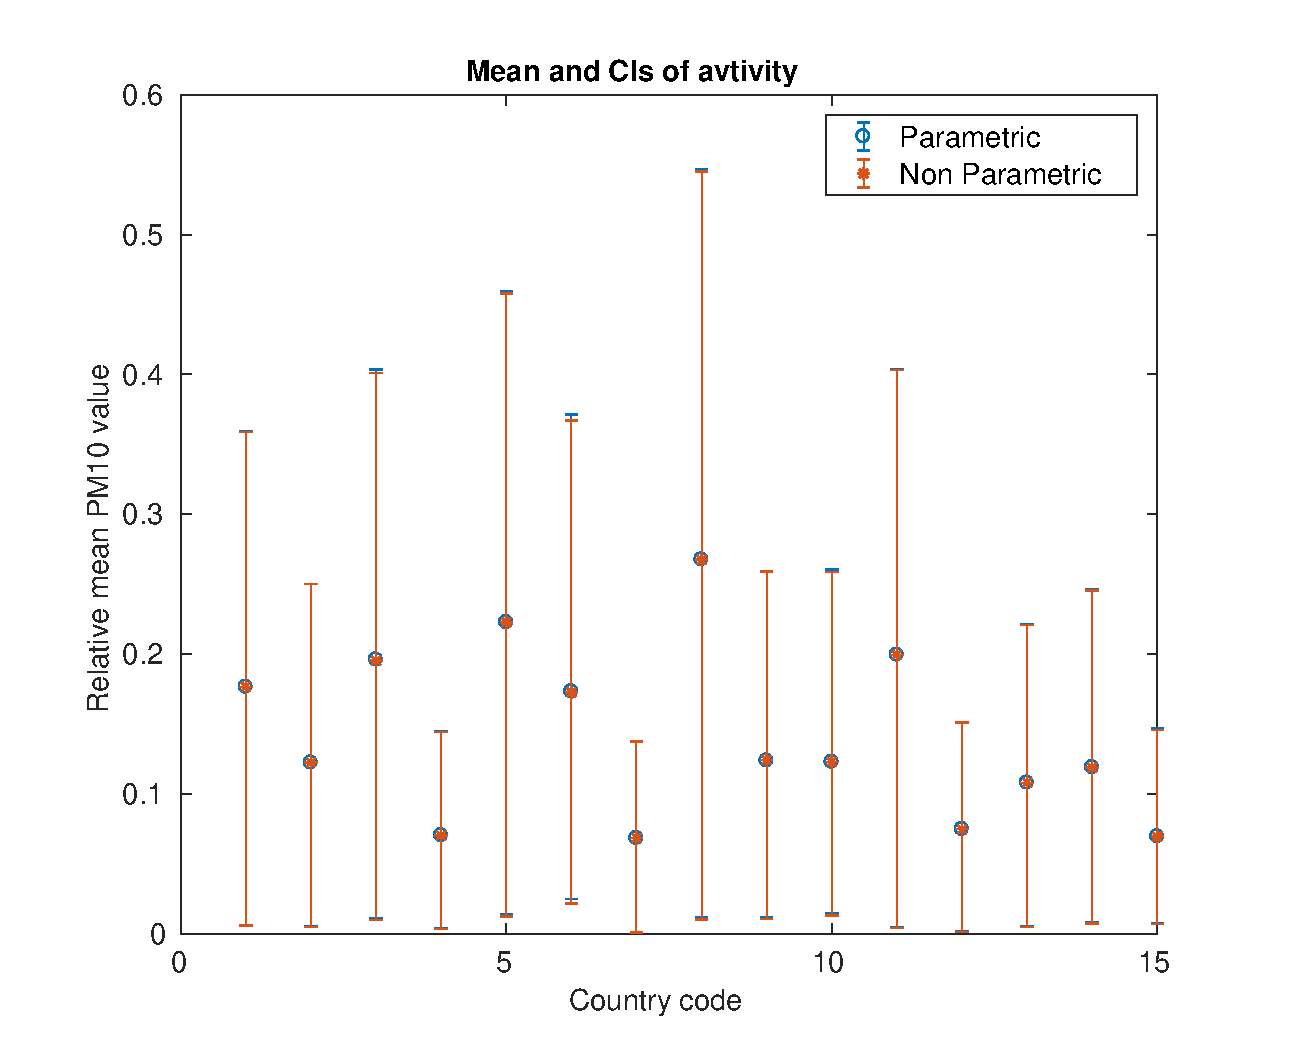
\includegraphics[width=1\columnwidth]{Ex3/Agriculture.eps}	
\caption{Μέσες τιμές και παραμετρικά και μη παραμετρικά διαστήματα για την δραστηριότητα Agriculture σε κάθε χώρα.}
\end{figure}

\begin{figure}[H]
\label{fig:z32} 
	\centering
	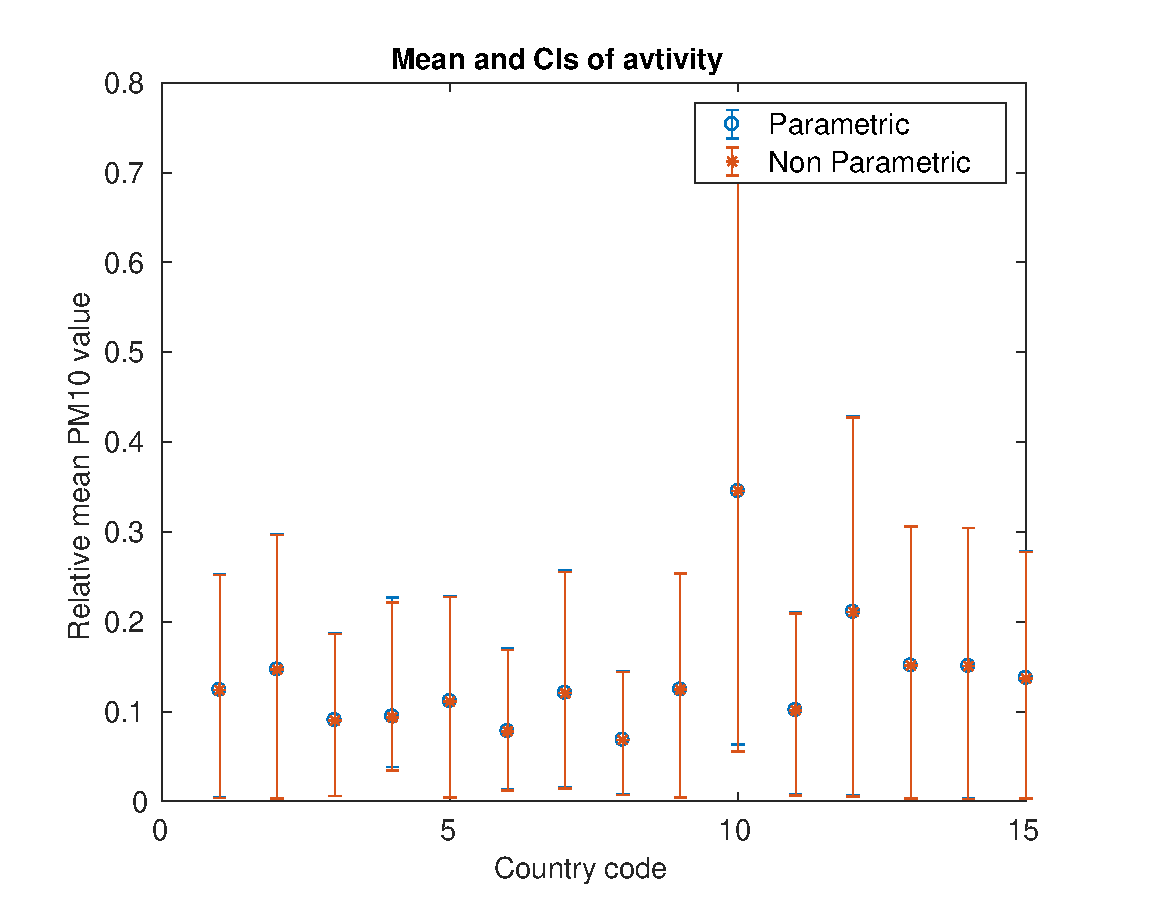
\includegraphics[width=1\columnwidth]{Ex3/IndustryEnergy.eps}	
\caption{Μέσες τιμές και παραμετρικά και μη παραμετρικά διαστήματα για την δραστηριότητα IndustryEnergy σε κάθε χώρα.}
\end{figure}

\begin{figure}[H]
\label{fig:z33} 
	\centering
	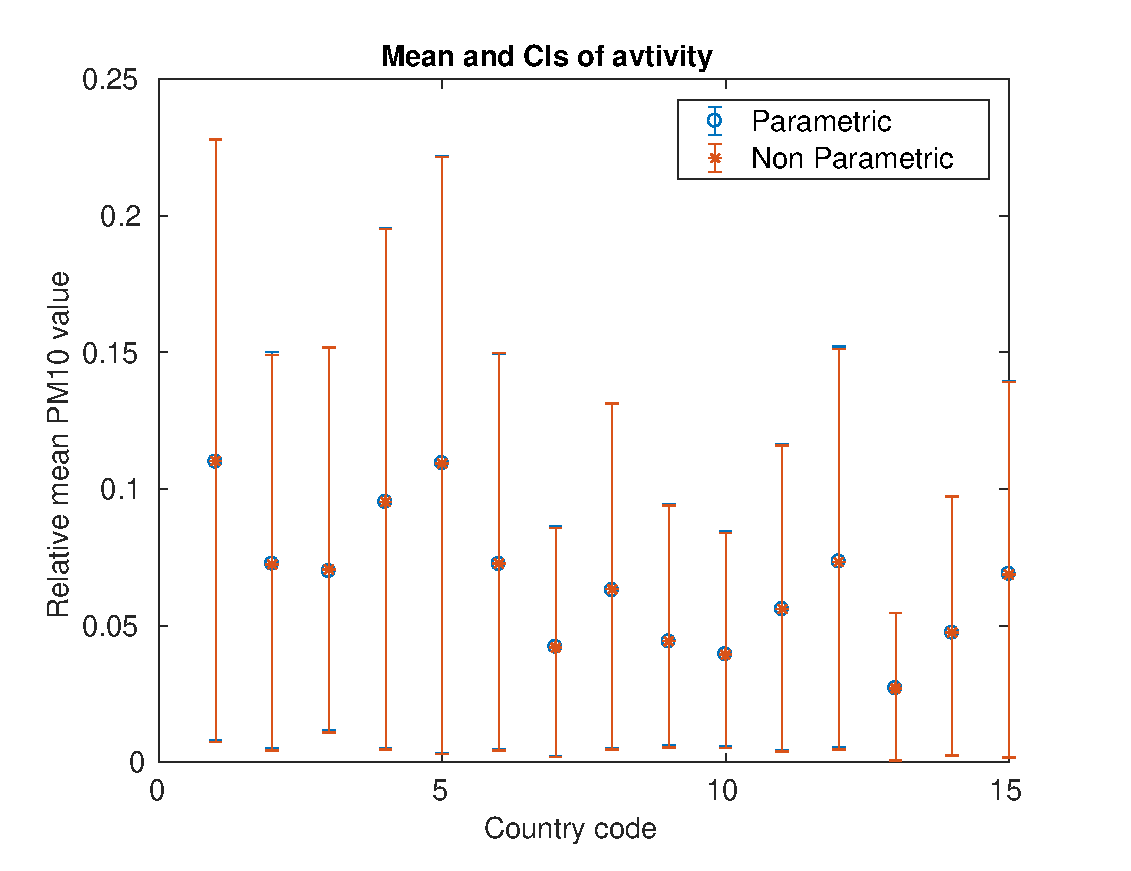
\includegraphics[width=1\columnwidth]{Ex3/OtherEnergy.eps}	
\caption{Μέσες τιμές και παραμετρικά και μη παραμετρικά διαστήματα για την δραστηριότητα OtherEnergy σε κάθε χώρα.}
\end{figure}

\begin{figure}[H]
\label{fig:z34} 
	\centering
	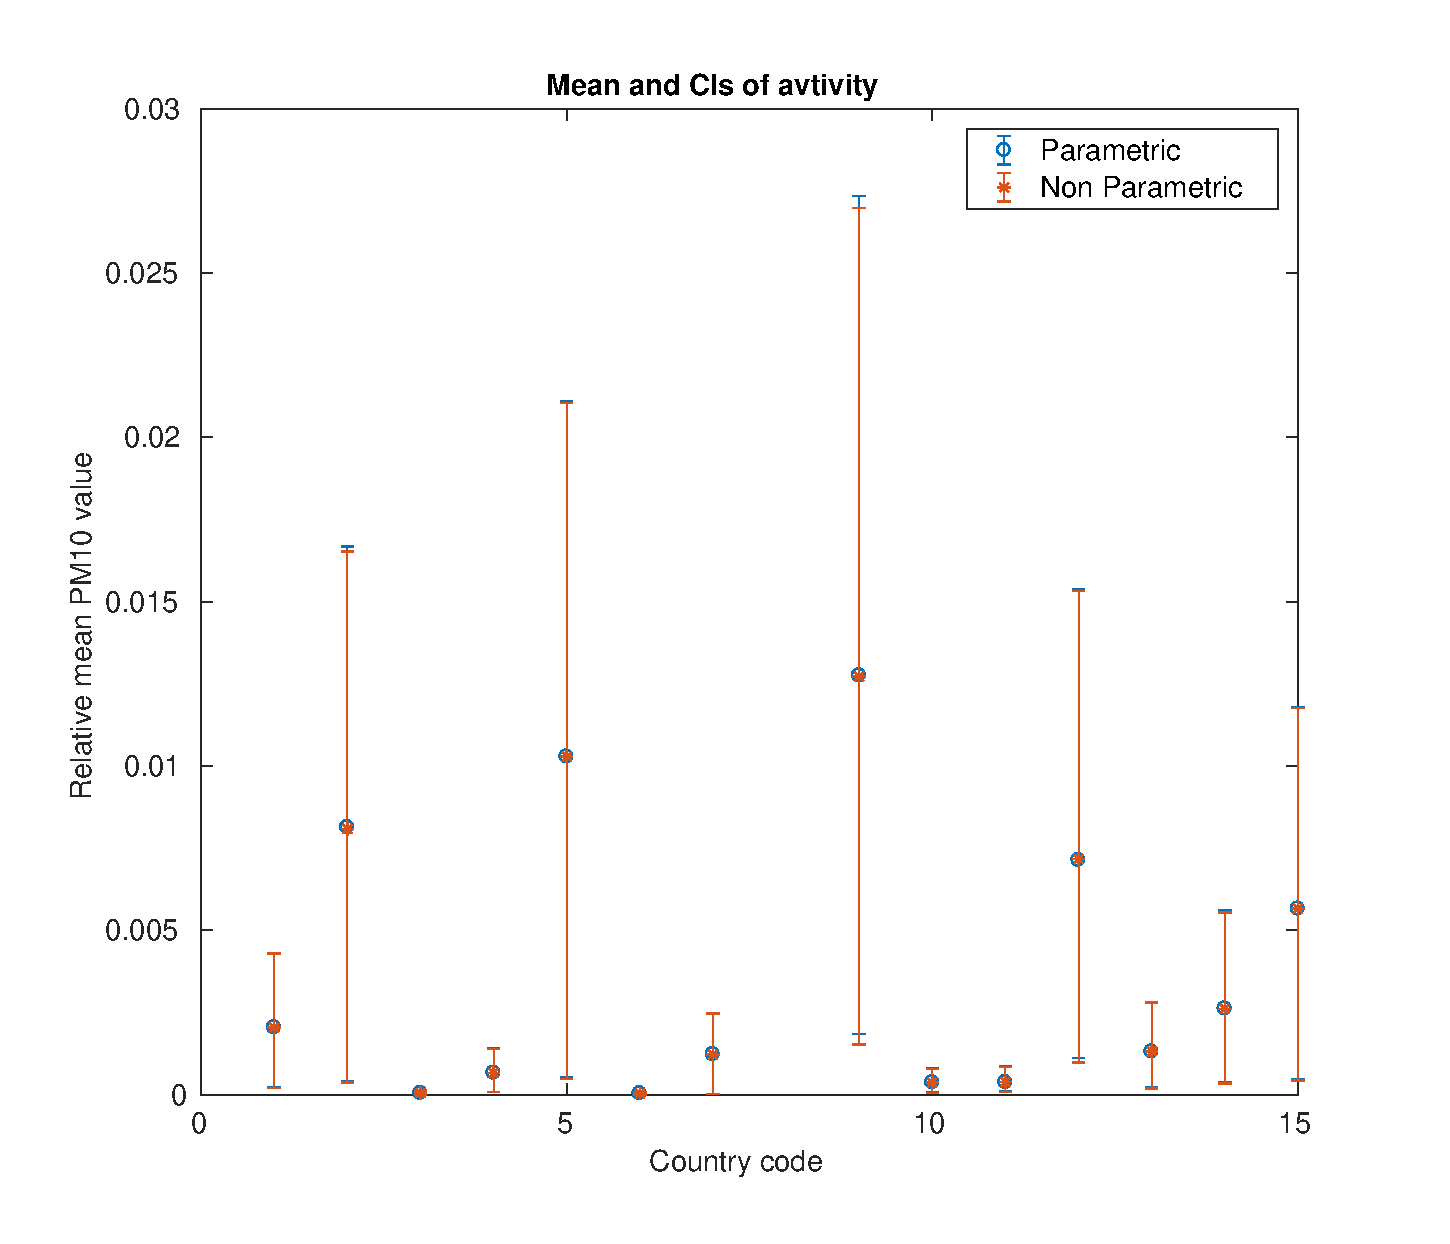
\includegraphics[width=1\columnwidth]{Ex3/Waste.eps}	
\caption{Μέσες τιμές και παραμετρικά και μη παραμετρικά διαστήματα για την δραστηριότητα Waste σε κάθε χώρα.}
\end{figure}


Από τα παραπάνω σχήματα δεν φαίνεται να υπάρχει μεγάλη διαφορά μεταξύ των μέσων τιμών και των διαστημάτων εμπιστοσύνης που προέρχονται από παραμετρική και με παραμετρική εκτίμηση.

\subsection{Ζήτημα 4}
\label{subsec:z4}

Η ίδια ανάλυση όπως και στο \hyperref[subsec:z3]{Κεφάλαιο \ref*{subsec:ze}} αλλά τώρα για την τυπική απόκλιση. Η ανάλυση γίνεται με τον \hyperref[mat:4]{κώδικα \ref*{mat:4}}. Καλέσαμε τον παραπάνω κώδιακ ενδεικτικά για μερικές δραστηριότητες και πήραμε τα παρακάτω \hyperref[fig:z41]{σχήμα \ref*{fig:z41}},\hyperref[fig:z42]{σχήμα \ref*{fig:z42}},\hyperref[fig:z43]{σχήμα \ref*{fig:z43}} και \hyperref[fig:z44]{σχήμα \ref*{fig:z44}}.

\begin{figure}[H]
\label{fig:z41} 
	\centering
	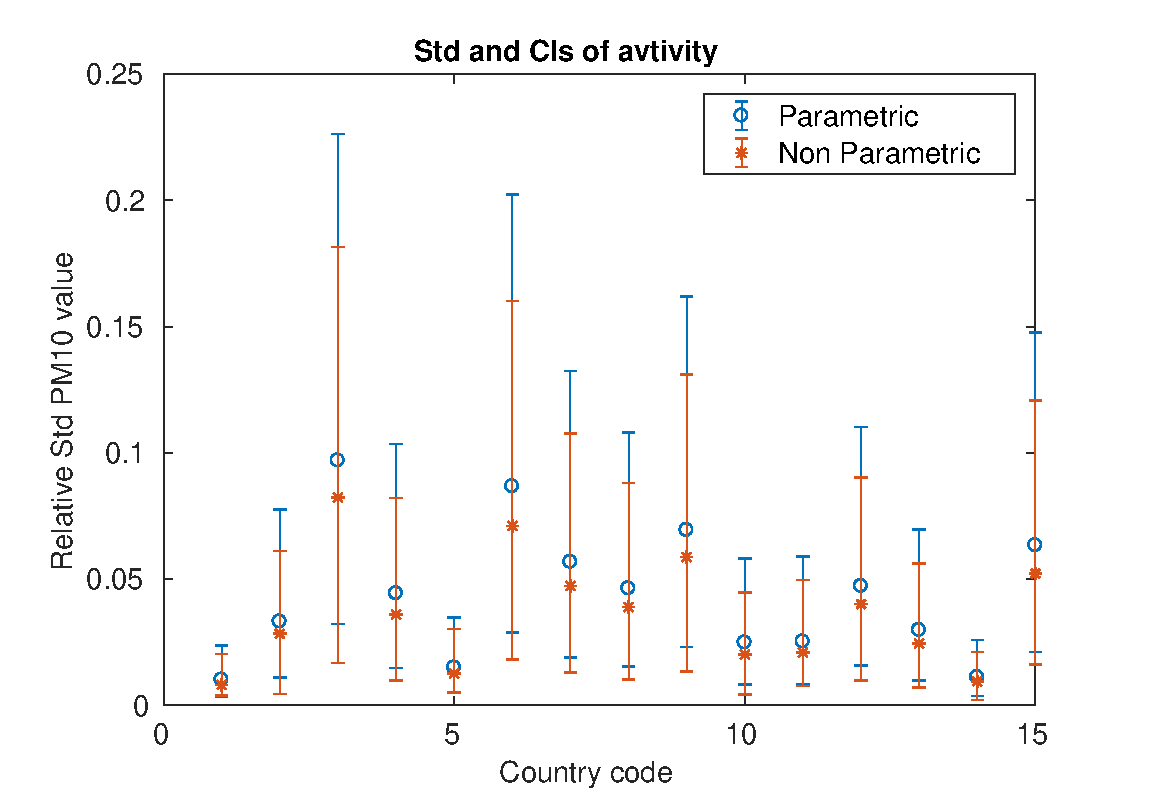
\includegraphics[width=1\columnwidth]{Ex4/EnergyIndustries.eps}	
\caption{Μέσες τιμές και παραμετρικά και μη παραμετρικά διαστήματα της τυπικής απόκλισης για την δραστηριότητα EnergyIndustries σε κάθε χώρα.}
\end{figure}

\begin{figure}[H]
\label{fig:z42} 
	\centering
	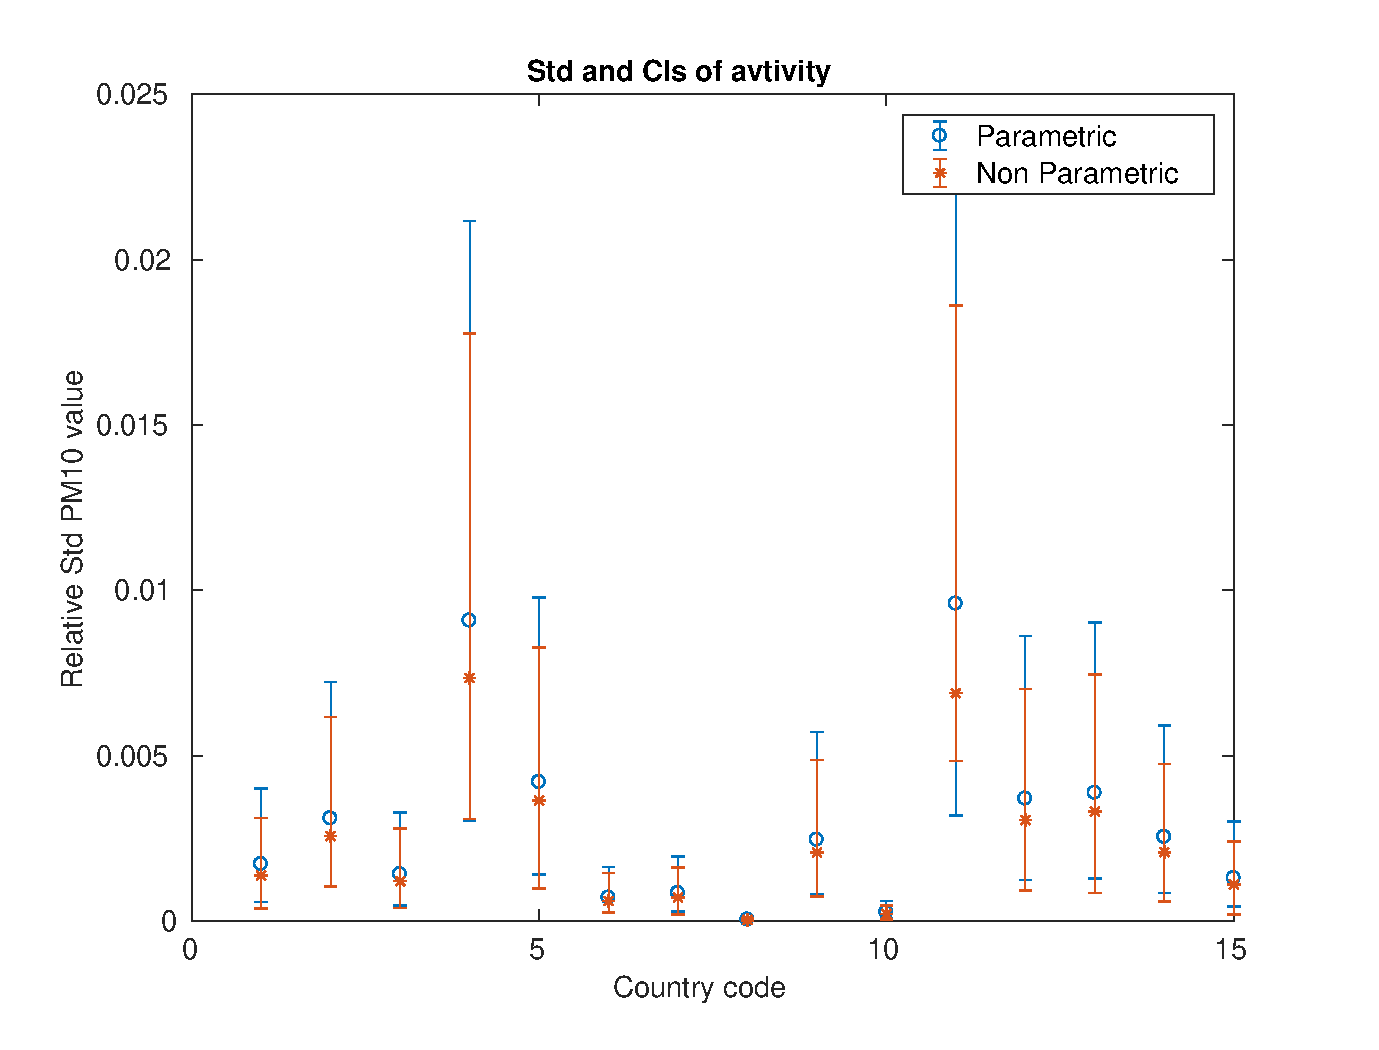
\includegraphics[width=1\columnwidth]{Ex4/FugitiveEmissions.eps}	
\caption{Μέσες τιμές και παραμετρικά και μη παραμετρικά διαστήματα της τυπικής απόκλισης για την δραστηριότητα FugitiveEmissions σε κάθε χώρα.}
\end{figure}

\begin{figure}[H]
\label{fig:z43} 
	\centering
	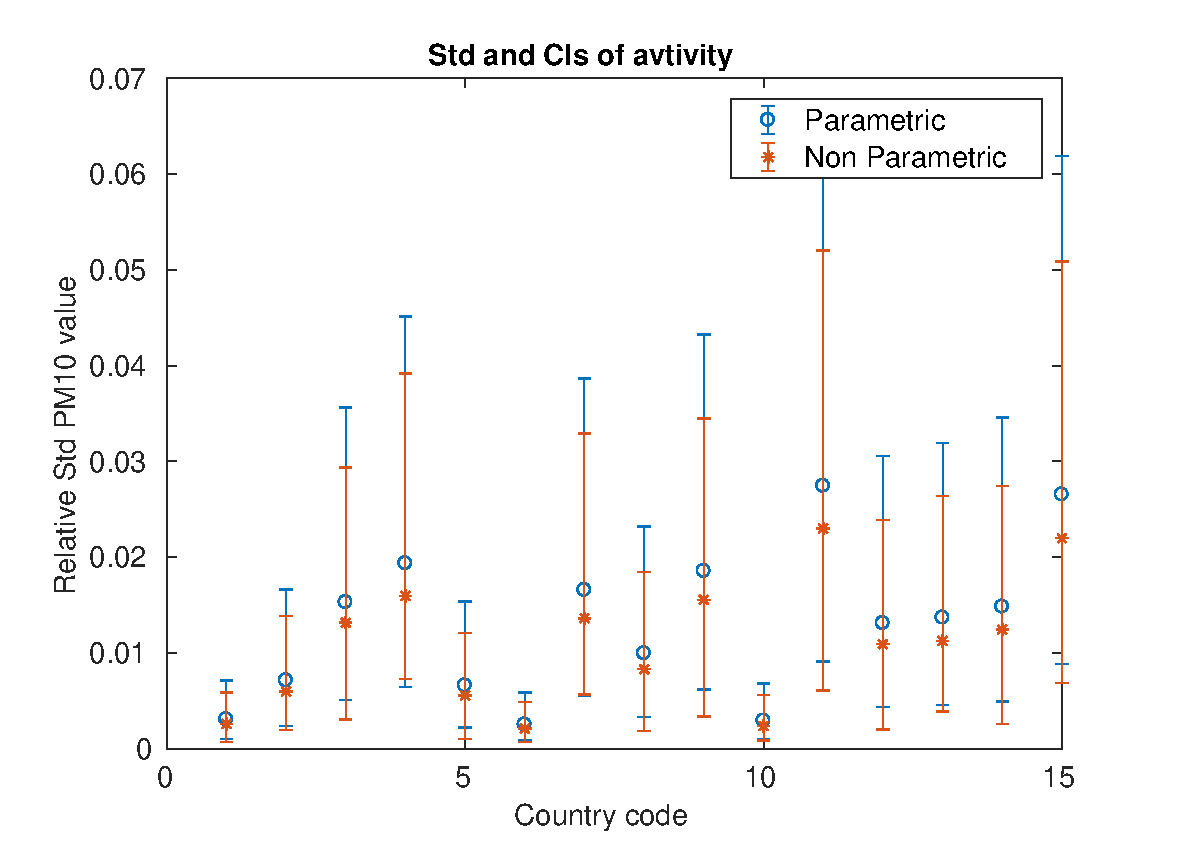
\includegraphics[width=1\columnwidth]{Ex4/OtherTransport.eps}	
\caption{Μέσες τιμές και παραμετρικά και μη παραμετρικά διαστήματα της τυπικής απόκλισης για την δραστηριότητα Othertransport σε κάθε χώρα.}
\end{figure}

\begin{figure}[H]
\label{fig:z44} 
	\centering
	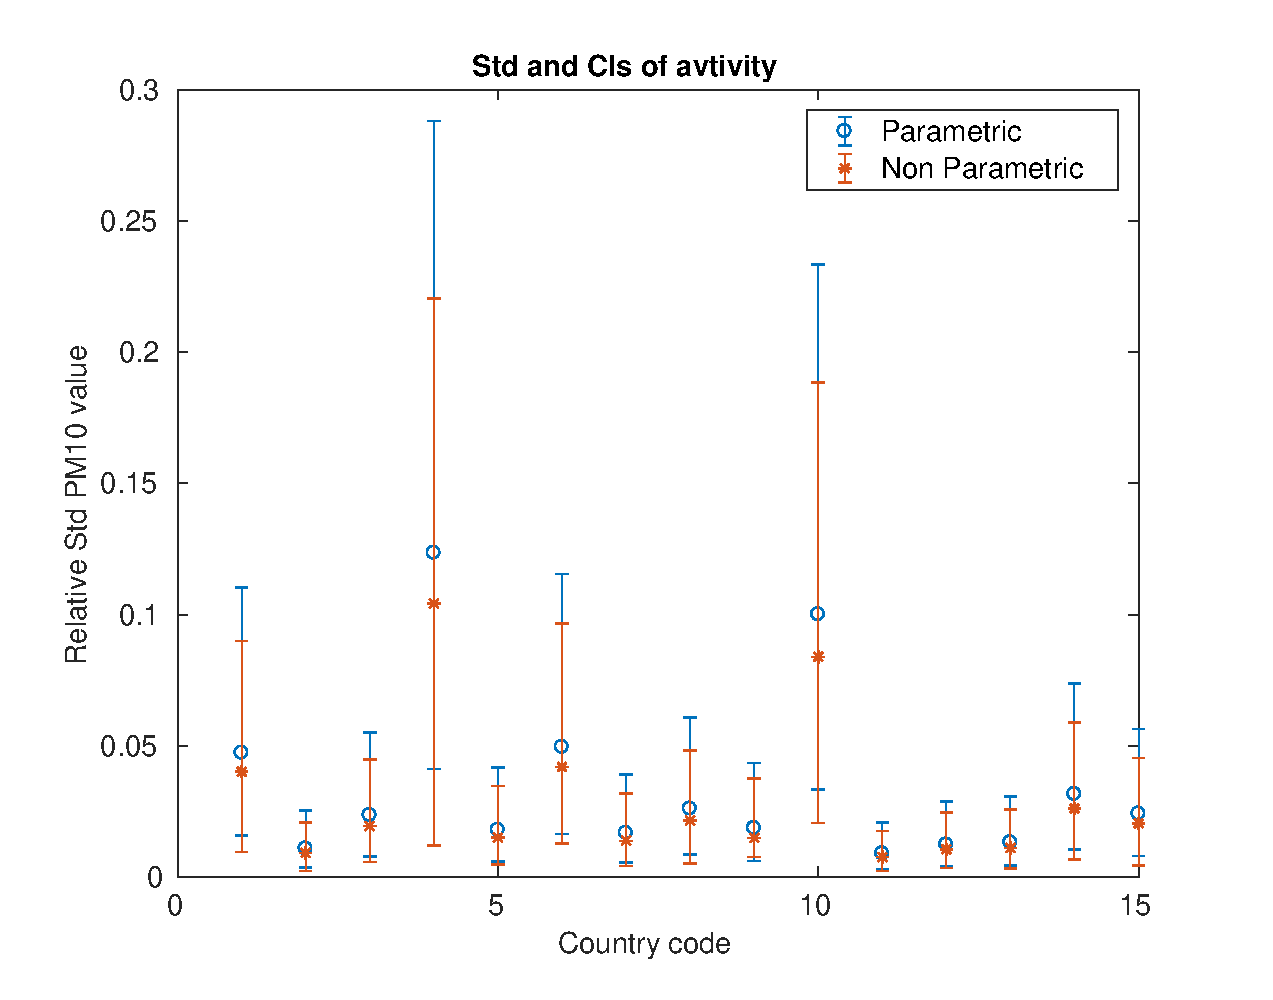
\includegraphics[width=1\columnwidth]{Ex4/RoadTransport.eps}	
\caption{Μέσες τιμές και παραμετρικά και μη παραμετρικά διαστήματα της τυπικής απόκλισης για την δραστηριότητα RoadTransport σε κάθε χώρα.}
\end{figure}

Από τα παραπάνω σχήματα παρατηρούμε ότι η μέσες τιμές της τυπικής απόκλισης διαφέρουν ανάμεσα στον παραμετρικό και μη τρόπο υπολογισμού τους. Καθώς και ότι σε γενικές γραμμές τα μη παραμετρικά διαστήματα εμπιστοσύνης είναι μικρότερα από τα αντίστοιχα παραμετρικά. Αυτό μπορεί να οφείλεται στον μεγάλο αριθμό (1000) τυχαίων δειγμάτων που δημιουργήσαμε στην μη παραμετρική ανάλυσή μας.  

\subsection{Ζήτημα 5}
\label{subsec:z5}

Για την επίλυση αυτού του ζητήματος κάνουμε χρήση του \hyperref[mat:5]{κώδικα \ref*{mat:5}}. Κατά την διάρκεια εκτέλεσης του κώδικα το Matlab επιστρέφει ένα γράφημα και τα αποτελέσματα του τεστ στην οθόνη. Ενδεικτικά καλέσαμε τον παραπάνω κώδικα για 4 δραστηριότητες και τα αποτελέσματα είναι παρακάτω.




\begin{figure}[H]
\label{fig:z51} 
	\centering
	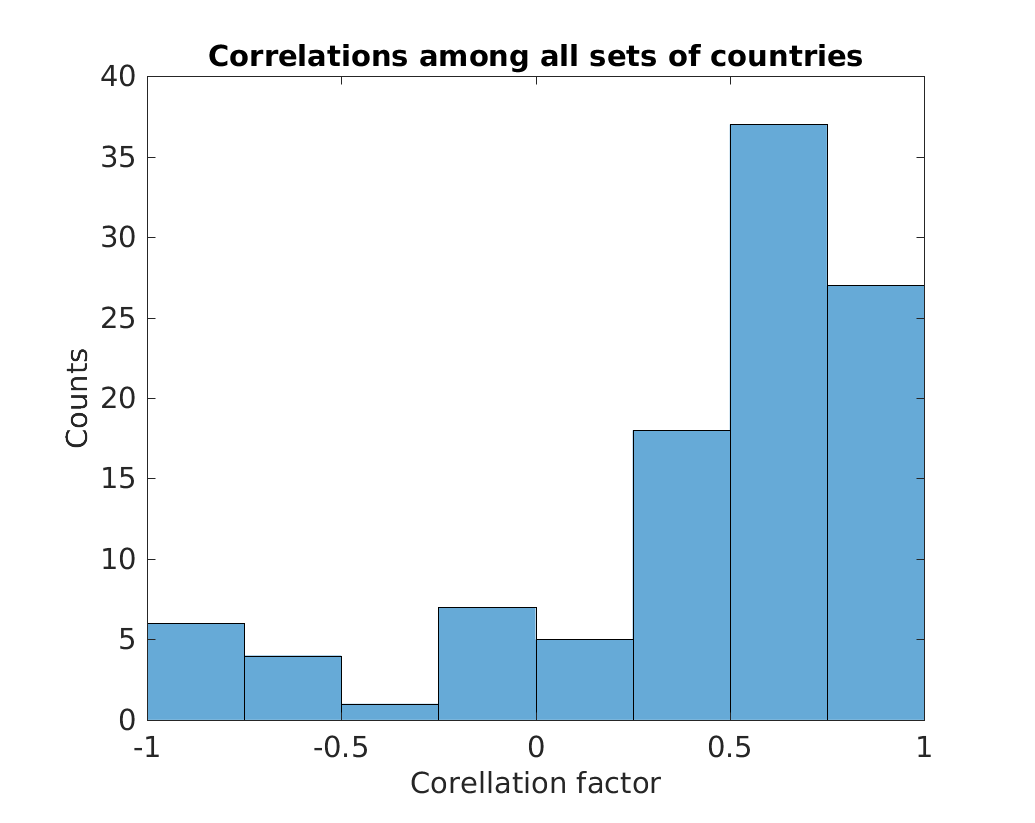
\includegraphics[width=1\columnwidth]{Ex5/Agriculture.eps}	
\caption{Ιστόγραμμα των συντελεστών συσχέτισης της δραστηριότητας Agriculture.}
\end{figure}



\begin{verbatim}
The 10 sets of countries with the highest 
correlation for Agriculture are
Correlation	 Country1	 Country2
 0.98	 	    Denmark	      Italy 
 0.97	 	 Netherlands	 United Kingdom 
 0.95	 	    Denmark	 Netherlands 
 0.95	 	      Italy	 United Kingdom 
 0.94	 	      Italy	 Netherlands 
 0.94	 	    Austria	    Belgium 
 0.94	 	    Denmark	 United Kingdom 
 0.91	 	    Belgium	 United Kingdom 
 0.91	 	    Austria	 Luxembourg 
 0.91	 	    Austria	 United Kingdom 

 29.52% of the sets of countries pass 
the Parametric test with a significance level of  5.00%

 25.71% of the sets of countries pass 
the NON-Parametric test with a significance level of  5.00%
\end{verbatim}



\begin{figure}[H]
\label{fig:z52} 
	\centering
	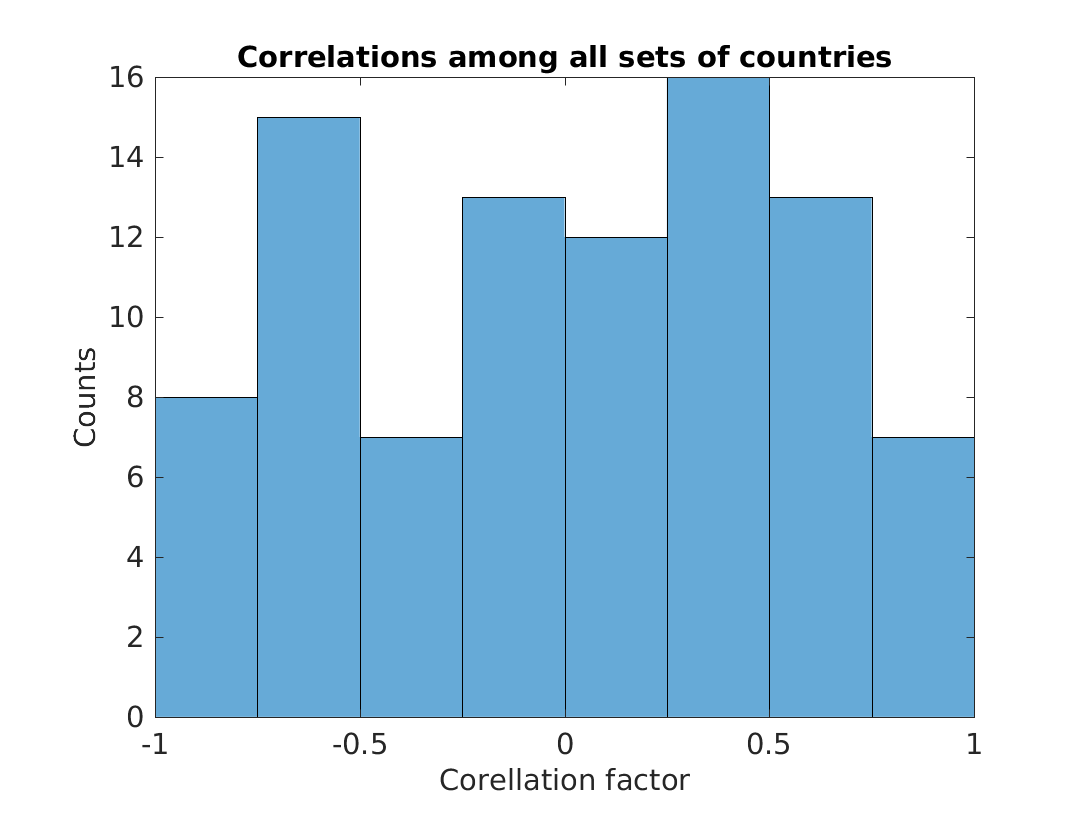
\includegraphics[width=1\columnwidth]{Ex5/Waste.eps}	
\caption{Ιστόγραμμα των συντελεστών συσχέτισης της δραστηριότητας Waste.}
\end{figure}



\begin{verbatim}
The 10 sets of countries with the highest 
correlation for Waste are
Correlation	 Country1	 Country2
  NaN	 	    Austria	    Ireland 
  NaN	 	    Belgium	    Ireland 
  NaN	 	    Denmark	    Ireland 
  NaN	 	    Finland	    Ireland 
  NaN	 	     France	    Ireland 
  NaN	 	    Germany	    Ireland 
  NaN	 	     Greece	    Ireland 
  NaN	 	    Ireland	      Italy 
  NaN	 	    Ireland	 Luxembourg 
  NaN	 	    Ireland	 Netherlands 

 44.76% of the sets of countries pass 
the Parametric test with a significance level of  5.00%

 57.14% of the sets of countries pass 
the NON-Parametric test with a significance level of  5.00%
\end{verbatim}




\begin{figure}[H]
\label{fig:z53} 
	\centering
	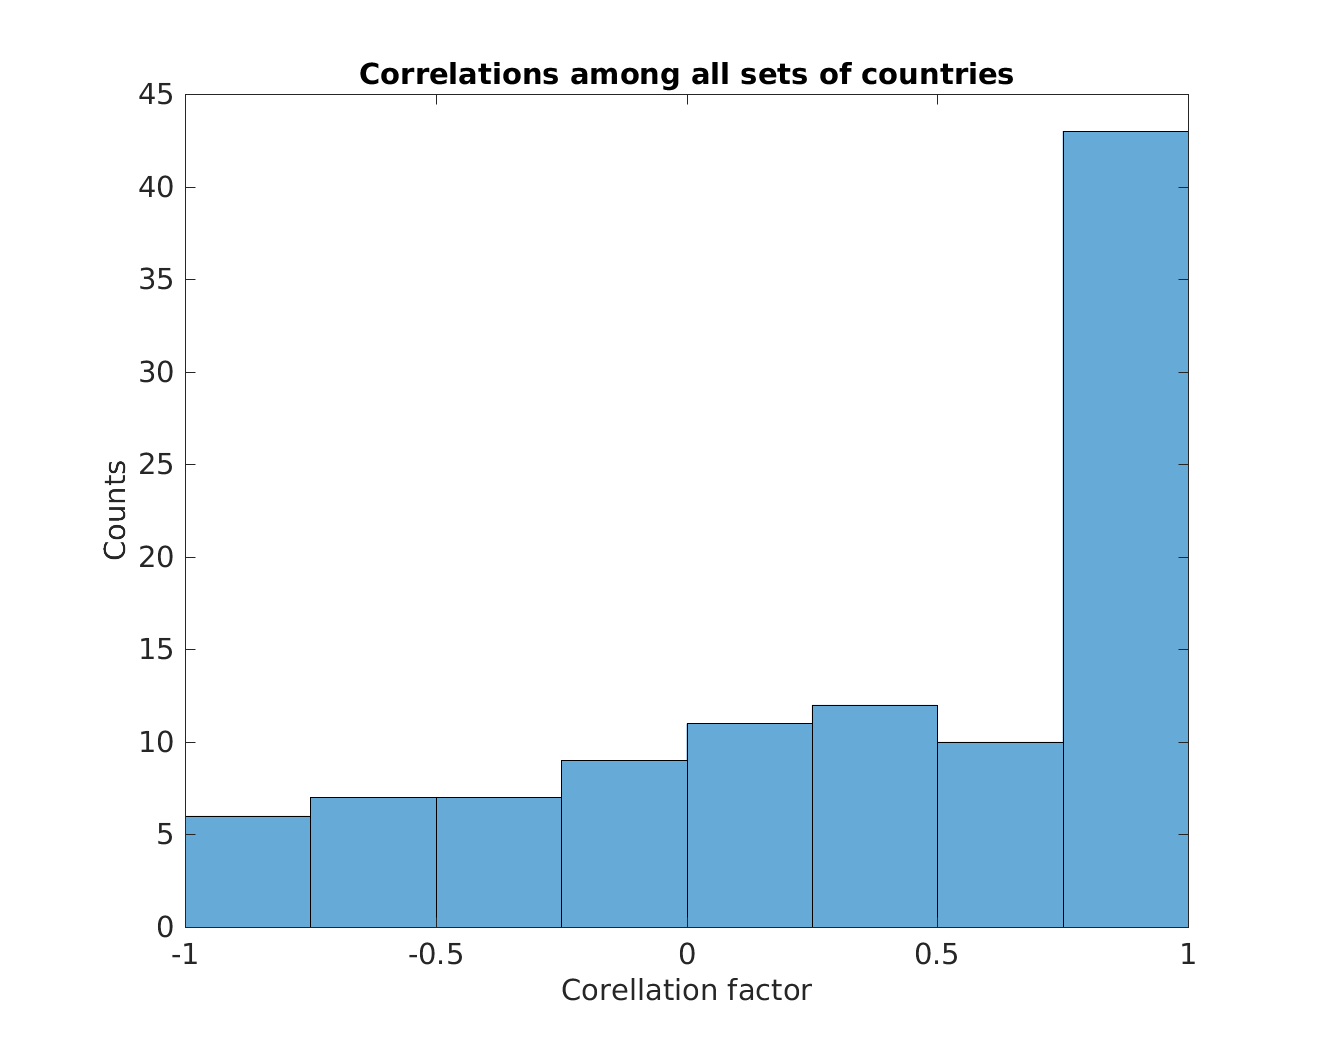
\includegraphics[width=1\columnwidth]{Ex5/IndustryEnergy.eps}	
\caption{Ιστόγραμμα των συντελεστών συσχέτισης της δραστηριότητας IndustryEnergy.}
\end{figure}



\begin{verbatim}
The 10 sets of countries with the highest 
correlation for IndustryEnergy are
Correlation	 Country1	 Country2
 0.99	 	     France	      Italy 
 0.98	 	 Luxembourg	 United Kingdom 
 0.97	 	      Italy	 Luxembourg 
 0.97	 	     France	 United Kingdom 
 0.97	 	    Belgium	 United Kingdom 
 0.97	 	      Italy	 United Kingdom 
 0.97	 	     France	 Luxembourg 
 0.97	 	     Sweden	 United Kingdom 
 0.96	 	    Belgium	      Italy 
 0.96	 	     France	     Sweden 

 35.24% of the sets of countries pass 
the Parametric test with a significance level of  5.00%

 33.33% of the sets of countries pass 
the NON-Parametric test with a significance level of  5.00%
\end{verbatim}


\begin{figure}[H]
\label{fig:z54} 
	\centering
	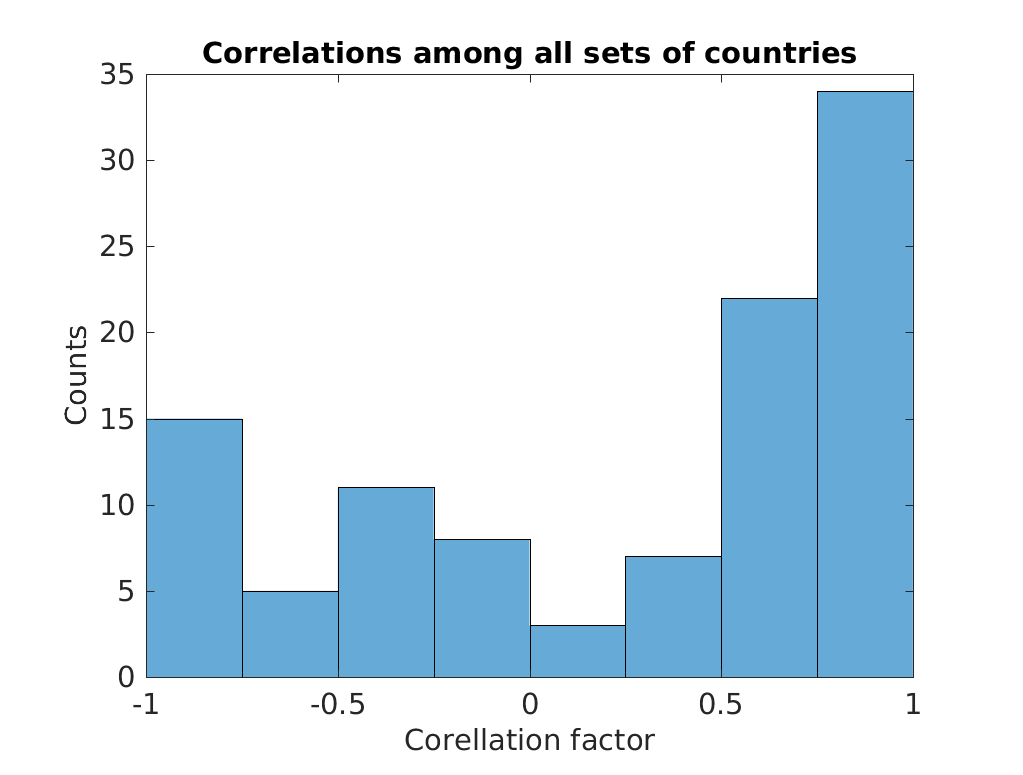
\includegraphics[width=1\columnwidth]{Ex5/RoadTransport.eps}	
\caption{Ιστόγραμμα των συντελεστών συσχέτισης της δραστηριότητας RoadTransport.}
\end{figure}



\begin{verbatim}
The 10 sets of countries with the highest 
correlation for RoadTransport are
Correlation	 Country1	 Country2
 1.00	 	    Denmark	 United Kingdom 
 0.99	 	    Denmark	     France 
 0.99	 	    Belgium	     France 
 0.99	 	    Denmark	     Sweden 
 0.99	 	    Germany	 United Kingdom 
 0.99	 	     France	 United Kingdom 
 0.99	 	     France	      Italy 
 0.99	 	     Sweden	 United Kingdom 
 0.99	 	     France	     Sweden 
 0.99	 	    Denmark	      Italy 

 25.71% of the sets of countries pass 
the Parametric test with a significance level of  5.00%

 25.71% of the sets of countries pass 
the NON-Parametric test with a significance level of  5.00%
\end{verbatim}











\subsection{Ζήτημα 6}
\label{subsec:z6}

Για την επίλυση αυτού του ζητήματος κάνουμε χρήση του \hyperref[mat:6]{κώδικα \ref*{mat:6}}.

\begin{figure}[H]
\label{fig:z61} 
	\centering
	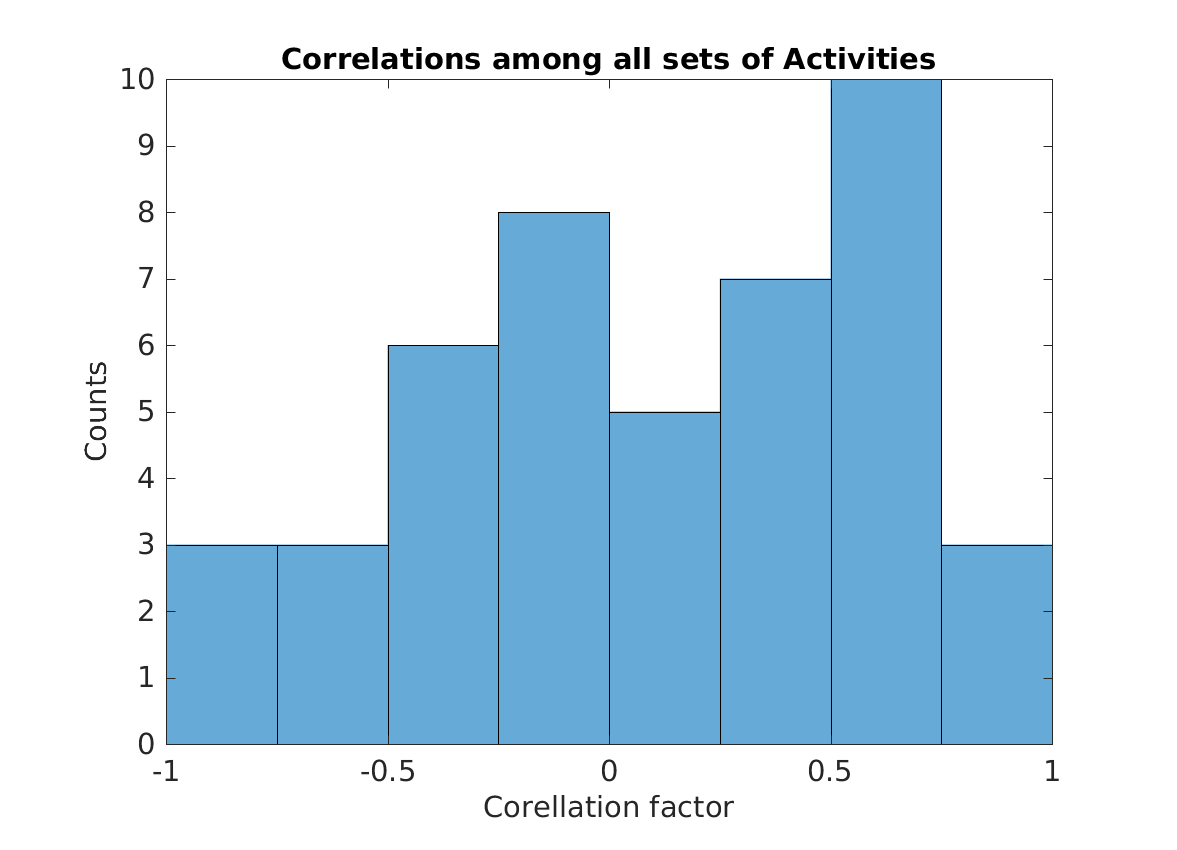
\includegraphics[width=1\columnwidth]{Ex6/Austria.eps}	
\caption{Ιστόγραμμα των συντελεστών συσχέτισης για την Austria.}
\end{figure}



\begin{verbatim}
The 10 sets of Activities with the highest correlation for Austria are
Correlation	 Activity1	 	 Activity2
 1.00	     EnergyIndustries	 	 EnergyIndustriesPowerProduction1A1a 
 0.82	    FugitiveEmissions	 	          OtherEnergy 
 0.76	        RoadTransport	 	                Waste 
 0.75	 EnergyIndustriesPowerProduction1A1a	 	       IndustryEnergy 
 0.74	 EnergyIndustriesPowerProduction1A1a	 	    IndustryProcesses 
 0.74	     EnergyIndustries	 	    IndustryProcesses 
 0.72	     EnergyIndustries	 	       IndustryEnergy 
 0.70	    IndustryProcesses	 	          OtherEnergy 
 0.70	          Agriculture	 	          OtherEnergy 
 0.64	 EnergyIndustriesPowerProduction1A1a	 	          OtherEnergy 

 53.33% of the sets of Activities pass 
the Parametric test with a significance level of  5.00%

 53.33% of the sets of Activities pass 
the NON-Parametric test with a significance level of  5.00%
\end{verbatim}


\begin{figure}[H]
\label{fig:z62} 
	\centering
	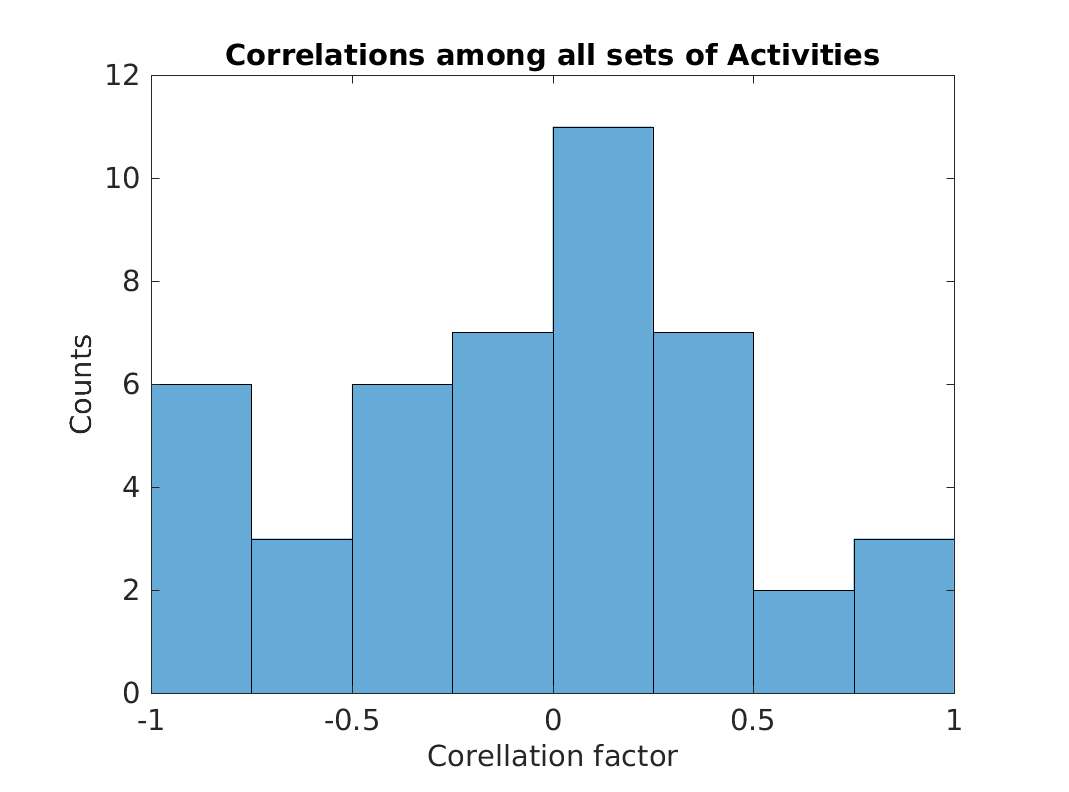
\includegraphics[width=1\columnwidth]{Ex6/Spain.eps}	
\caption{Ιστόγραμμα των συντελεστών συσχέτισης για την Spain.}
\end{figure}



\begin{verbatim}
The 10 sets of Activities with the highest correlation for Spain are
Correlation	 Activity1	 	 Activity2
 0.99	     EnergyIndustries	 	 EnergyIndustriesPowerProduction1A1a 
 0.92	       OtherTransport	 	                Waste 
 0.77	    FugitiveEmissions	 	        RoadTransport 
 0.66	          Agriculture	 	       OtherTransport 
 0.55	     EnergyIndustries	 	    FugitiveEmissions 
 0.48	          Agriculture	 	                Waste 
 0.46	 EnergyIndustriesPowerProduction1A1a	 	    FugitiveEmissions 
 0.44	     EnergyIndustries	 	        RoadTransport 
 0.35	 EnergyIndustriesPowerProduction1A1a	 	        RoadTransport 
 0.32	          OtherEnergy	 	        RoadTransport 

 64.44% of the sets of Activities pass 
the Parametric test with a significance level of  5.00%

 62.22% of the sets of Activities pass 
the NON-Parametric test with a significance level of  5.00%
\end{verbatim}


\begin{figure}[H]
\label{fig:z6} 
	\centering
	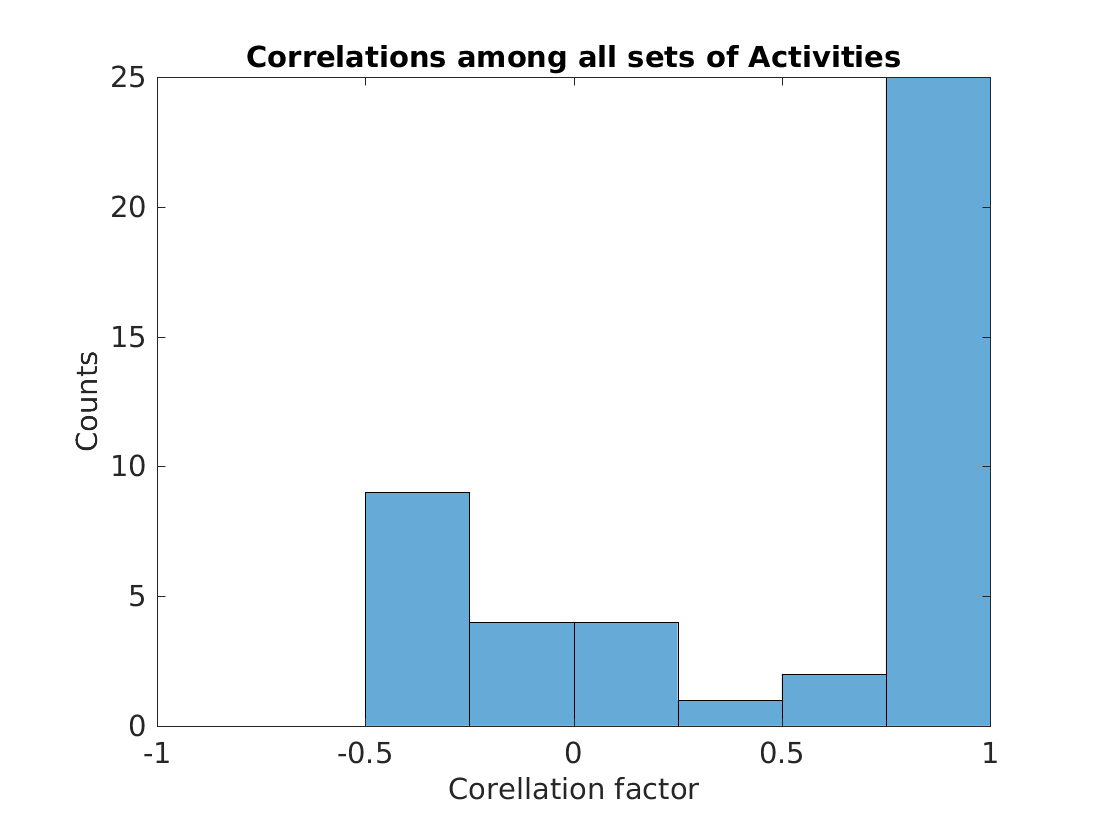
\includegraphics[width=1\columnwidth]{Ex6/Italy.eps}	
\caption{Ιστόγραμμα των συντελεστών συσχέτισης για την Italy.}
\end{figure}



\begin{verbatim}

The 10 sets of Activities with the highest correlation for Italy are
Correlation	 Activity1	 	 Activity2
 1.00	     EnergyIndustries	 	 EnergyIndustriesPowerProduction1A1a 
 0.97	     EnergyIndustries	 	        RoadTransport 
 0.96	 EnergyIndustriesPowerProduction1A1a	 	        RoadTransport 
 0.96	     EnergyIndustries	 	       IndustryEnergy 
 0.96	 EnergyIndustriesPowerProduction1A1a	 	       IndustryEnergy 
 0.95	          Agriculture	 	     EnergyIndustries 
 0.95	          Agriculture	 	 EnergyIndustriesPowerProduction1A1a 
 0.93	          Agriculture	 	        RoadTransport 
 0.92	          Agriculture	 	       IndustryEnergy 
 0.91	       IndustryEnergy	 	        RoadTransport 

 40.00% of the sets of Activities pass 
the Parametric test with a significance level of  5.00%

 37.78% of the sets of Activities pass 
the NON-Parametric test with a significance level of  5.00%
\end{verbatim}



\begin{figure}[H]
\label{fig:z6} 
	\centering
	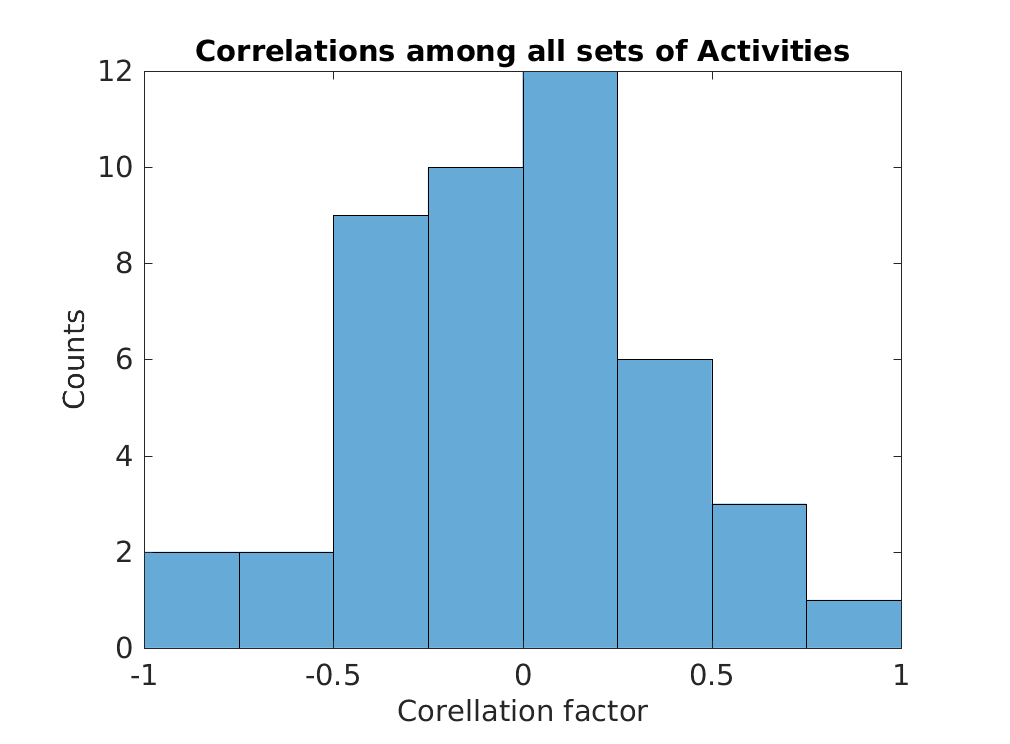
\includegraphics[width=1\columnwidth]{Ex6/Greece.eps}	
\caption{Ιστόγραμμα των συντελεστών συσχέτισης για την Greece.}
\end{figure}



\begin{verbatim}
The 10 sets of Activities with the highest correlation for Greece are
Correlation	 Activity1	 	 Activity2
 1.00	     EnergyIndustries	 	 EnergyIndustriesPowerProduction1A1a 
 0.65	       IndustryEnergy	 	    IndustryProcesses 
 0.59	          Agriculture	 	       IndustryEnergy 
 0.54	          Agriculture	 	    IndustryProcesses 
 0.49	       IndustryEnergy	 	        RoadTransport 
 0.45	          OtherEnergy	 	        RoadTransport 
 0.37	          Agriculture	 	        RoadTransport 
 0.32	       IndustryEnergy	 	          OtherEnergy 
 0.32	       OtherTransport	 	        RoadTransport 
 0.29	          OtherEnergy	 	       OtherTransport 

 77.78% of the sets of Activities pass 
the Parametric test with a significance level of  5.00%

 75.56% of the sets of Activities pass 
the NON-Parametric test with a significance level of  5.00%
\end{verbatim}






\subsection{Ζήτημα 7}
\label{subsec:z7}

\subsection{Ζήτημα 8}
\label{subsec:z8}

\subsection{Ζήτημα 9}
\label{subsec:z9}

\subsection{Ζήτημα 10}
\label{subsec:z10}



\section{Προγράμματα}
\label{sec:Prog}
Στο κεφάλαιο αυτό παραθέτονται οι κώδικες σε γλώσσα Matlab που χρησιμοποιήθηκαν για την επίλυση των παραπάνω ζητημάτων. Σε περίπτωση που  κώδικας καλεί επί μέρους συναρτήσεις αυτές αναφέρονται και παραθέτονται. 

\subsection{Exercise1}
\label{prog:1}
Πρόγραμμα Matlab για την επίλυση του \hyperref[subsection:z1]{Ζητούμενου \ref*{subsec:z1}}. Το οποίο με την σειρά του καλεί τα προγράμματα \hyperref[prog:DataLoader]{DataLoader} και \hyperref[prog:Chartme]{Chartme}.
\lstinputlisting[
	caption=Project2019Ex1.m, % Caption above the listing
	label=mat:1, % Label for referencing this listing
	language=Matlab, % Use Perl functions/syntax highlighting
	frame=single, % Frame around the code listing
	showstringspaces=false, % Don't put marks in string spaces
	numbers=left, % Line numbers on left
	numberstyle=\small, % Line numbers styling
	]{../ZagkourisProject2019Ex1.m}



\subsection{DataLoader}
\label{prog:DataLoader}
Πρόγραμμα για την επιλογή και εισαγωγή δεδομένων προς ανάλυση στο Matlab
\lstinputlisting[
	caption=Dataloader.m, % Caption above the listing
	label=mat:DataLoader, % Label for referencing this listing
	language=Matlab, % Use Perl functions/syntax highlighting
	frame=single, % Frame around the code listing
	showstringspaces=false, % Don't put marks in string spaces
	numbers=left, % Line numbers on left
	numberstyle=\small, % Line numbers styling
	]{../DataLoader.m}




\subsection{Chartme}
\label{prog:Chartme}
Πρόγραμμα για την δημιουργία Ιστογραμμάτων για το \hyperref[subsection:z1]{Ζητούμενου \ref*{subsec:z1}}.
\lstinputlisting[
	caption=Chartme.m, % Caption above the listing
	label=mat:Chartme, % Label for referencing this listing
	language=Matlab, % Use Perl functions/syntax highlighting
	frame=single, % Frame around the code listing
	showstringspaces=false, % Don't put marks in string spaces
	numbers=left, % Line numbers on left
	numberstyle=\small, % Line numbers styling
	]{../Chartme.m}


\subsection{Exercise2}
\label{prog:2}
Πρόγραμμα Matlab για την επίλυση του \hyperref[subsection:z2]{Ζητούμενου \ref*{subsec:z2}}. Το οποίο με την σειρά του καλεί το προγράμμα \hyperref[prog:DataLoader]{DataLoader}.
\lstinputlisting[
	caption=Project2019Ex2.m, % Caption above the listing
	label=mat:2, % Label for referencing this listing
	language=Matlab, % Use Perl functions/syntax highlighting
	frame=single, % Frame around the code listing
	showstringspaces=false, % Don't put marks in string spaces
	numbers=left, % Line numbers on left
	numberstyle=\small, % Line numbers styling
	]{../ZagkourisProject2019Ex2.m}


\subsection{Exercise3}
\label{prog:3}
Πρόγραμμα Matlab για την επίλυση του \hyperref[subsection:z3]{Ζητούμενου \ref*{subsec:z3}}. Το οποίο με την σειρά του καλεί το προγράμμα \hyperref[prog:DataLoader]{DataLoader}, \hyperref[prog:CIs]{CIs} και \hyperref[prog:MeanP10]{MeanP10}.
\lstinputlisting[
	caption=Project2019Ex3.m, % Caption above the listing
	label=mat:3, % Label for referencing this listing
	language=Matlab, % Use Perl functions/syntax highlighting
	frame=single, % Frame around the code listing
	showstringspaces=false, % Don't put marks in string spaces
	numbers=left, % Line numbers on left
	numberstyle=\small, % Line numbers styling
	]{../ZagkourisProject2019Ex3.m}

\subsection{CIs}
\label{prog:CIs}
Πρόγραμμα για τον υπολογισμό διαστημάτων εμπιστοσύνης για το \hyperref[subsection:z3]{Ζητούμενο \ref*{subsec:z3}}.
\lstinputlisting[
	caption=CIs.m, % Caption above the listing
	label=mat:CIs, % Label for referencing this listing
	language=Matlab, % Use Perl functions/syntax highlighting
	frame=single, % Frame around the code listing
	showstringspaces=false, % Don't put marks in string spaces
	numbers=left, % Line numbers on left
	numberstyle=\small, % Line numbers styling
	]{../CIs.m}

\subsection{MeanP10}
\label{prog:MeanP10}
Πρόγραμμα για τον υπολογισμό των μέσων τιμών για το \hyperref[subsection:z3]{Ζητούμενο \ref*{subsec:z3}}.
\lstinputlisting[
	caption=MeanP10.m, % Caption above the listing
	label=mat:MeanP10, % Label for referencing this listing
	language=Matlab, % Use Perl functions/syntax highlighting
	frame=single, % Frame around the code listing
	showstringspaces=false, % Don't put marks in string spaces
	numbers=left, % Line numbers on left
	numberstyle=\small, % Line numbers styling
	]{../MeanP10.m}
	
\subsection{Exercise4}
\label{prog:4}
Πρόγραμμα Matlab για την επίλυση του \hyperref[subsection:z4]{Ζητούμενου \ref*{subsec:z4}}. Το οποίο με την σειρά του καλεί το προγράμμα \hyperref[prog:DataLoader]{DataLoader}, \hyperref[prog:stdCIs]{stdCIs} και \hyperref[prog:StdP10]{StdP10}.
\lstinputlisting[
	caption=Project2019Ex4.m, % Caption above the listing
	label=mat:4, % Label for referencing this listing
	language=Matlab, % Use Perl functions/syntax highlighting
	frame=single, % Frame around the code listing
	showstringspaces=false, % Don't put marks in string spaces
	numbers=left, % Line numbers on left
	numberstyle=\small, % Line numbers styling
	]{../ZagkourisProject2019Ex4.m}

\subsection{stdCIs}
\label{prog:stdCIs}
Πρόγραμμα για τον υπολογισμό διαστημάτων εμπιστοσύνης για το \hyperref[subsection:z4]{Ζητούμενο \ref*{subsec:z4}}.
\lstinputlisting[
	caption=stdCIs.m, % Caption above the listing
	label=mat:stdCIs, % Label for referencing this listing
	language=Matlab, % Use Perl functions/syntax highlighting
	frame=single, % Frame around the code listing
	showstringspaces=false, % Don't put marks in string spaces
	numbers=left, % Line numbers on left
	numberstyle=\small, % Line numbers styling
	]{../stdCIs.m}

\subsection{StdP10}
\label{prog:StdP10}
Πρόγραμμα για τον υπολογισμό των μέσων τιμών για το \hyperref[subsection:z4]{Ζητούμενο \ref*{subsec:z4}}.
\lstinputlisting[
	caption=StdP10.m, % Caption above the listing
	label=mat:StdP10, % Label for referencing this listing
	language=Matlab, % Use Perl functions/syntax highlighting
	frame=single, % Frame around the code listing
	showstringspaces=false, % Don't put marks in string spaces
	numbers=left, % Line numbers on left
	numberstyle=\small, % Line numbers styling
	]{../StdP10.m}
	
	
	
\subsection{Exercise5}
\label{prog:5}
Πρόγραμμα Matlab για την επίλυση του \hyperref[subsection:z5]{Ζητούμενου \ref*{subsec:z5}}. Το οποίο με την σειρά του καλεί το προγράμμα \hyperref[prog:DataLoader]{DataLoader}, \hyperref[prog:AllCountries]{AllCountries} και \hyperref[prog:corrme]{corrme}.
\lstinputlisting[
	caption=Project2019Ex5.m, % Caption above the listing
	label=mat:5, % Label for referencing this listing
	language=Matlab, % Use Perl functions/syntax highlighting
	frame=single, % Frame around the code listing
	showstringspaces=false, % Don't put marks in string spaces
	numbers=left, % Line numbers on left
	numberstyle=\small, % Line numbers styling
	]{../ZagkourisProject2019Ex5.m}

\subsection{AllCountries}
\label{prog:AllCountries}
Πρόγραμμα για τον υπολογισμό διαστημάτων εμπιστοσύνης για το \hyperref[subsection:z5]{Ζητούμενο \ref*{subsec:z5}}.
\lstinputlisting[
	caption=AllCountries.m, % Caption above the listing
	label=mat:AllCountries, % Label for referencing this listing
	language=Matlab, % Use Perl functions/syntax highlighting
	frame=single, % Frame around the code listing
	showstringspaces=false, % Don't put marks in string spaces
	numbers=left, % Line numbers on left
	numberstyle=\small, % Line numbers styling
	]{../AllCountries.m}

\subsection{corrme}
\label{prog:corrme}
Πρόγραμμα για τον υπολογισμό των μέσων τιμών για το \hyperref[subsection:z5]{Ζητούμενο \ref*{subsec:z5}}.
\lstinputlisting[
	caption=corrme.m, % Caption above the listing
	label=mat:corrme, % Label for referencing this listing
	language=Matlab, % Use Perl functions/syntax highlighting
	frame=single, % Frame around the code listing
	showstringspaces=false, % Don't put marks in string spaces
	numbers=left, % Line numbers on left
	numberstyle=\small, % Line numbers styling
	]{../corrme.m}	
	
	
	
		
\subsection{Exercise6}
\label{prog:6}
Πρόγραμμα Matlab για την επίλυση του \hyperref[subsection:z6]{Ζητούμενου \ref*{subsec:z6}}. Το οποίο με την σειρά του καλεί το προγράμμα \hyperref[prog:DataLoader]{DataLoader}, \hyperref[prog:AllActivities]{AllActivities} και \hyperref[prog:corrme]{corrme}.
\lstinputlisting[
	caption=Project2019Ex6.m, % Caption above the listing
	label=mat:6, % Label for referencing this listing
	language=Matlab, % Use Perl functions/syntax highlighting
	frame=single, % Frame around the code listing
	showstringspaces=false, % Don't put marks in string spaces
	numbers=left, % Line numbers on left
	numberstyle=\small, % Line numbers styling
	]{../ZagkourisProject2019Ex6.m}

\subsection{AllActivities}
\label{prog:AllActivities}
Πρόγραμμα για τον υπολογισμό διαστημάτων εμπιστοσύνης για το \hyperref[subsection:z6]{Ζητούμενο \ref*{subsec:z6}}.
\lstinputlisting[
	caption=AllActivities.m, % Caption above the listing
	label=mat:AllActivities, % Label for referencing this listing
	language=Matlab, % Use Perl functions/syntax highlighting
	frame=single, % Frame around the code listing
	showstringspaces=false, % Don't put marks in string spaces
	numbers=left, % Line numbers on left
	numberstyle=\small, % Line numbers styling
	]{../AllActivities.m}
	
	
	
	
	
	
----------------------------------------------------------

\section{Understanding Text}


\subsubsection{Suppose ``chuck" implies throwing.}

According to the Associated Press (1988), a New York Fish and Wildlife technician named Richard Thomas calculated the volume of dirt in a typical 25--30 foot (7.6--9.1 m) long woodchuck burrow and had determined that if the woodchuck had moved an equivalent volume of wood, it could move ``about \textbf{700 pounds (320 kg)} on a good day, with the wind at his back".

%------------------------------------------------

\subsubsection{Suppose ``chuck" implies vomiting.}

A woodchuck can ingest 361.92 cm\textsuperscript{3} (22.09 cu in) of wood per day. Assuming immediate expulsion on ingestion with a 5\% retainment rate, a woodchuck could chuck \textbf{343.82 cm\textsuperscript{3}} of wood per day.

%------------------------------------------------

\paragraph{Bonus: suppose there is no woodchuck.}

Fusce varius orci ac magna dapibus porttitor. In tempor leo a neque bibendum sollicitudin. Nulla pretium fermentum nisi, eget sodales magna facilisis eu. Praesent aliquet nulla ut bibendum lacinia. Donec vel mauris vulputate, commodo ligula ut, egestas orci. Suspendisse commodo odio sed hendrerit lobortis. Donec finibus eros erat, vel ornare enim mattis et.

%----------------------------------------------------------------------------------------
%	EQUATION EXAMPLES
%----------------------------------------------------------------------------------------

\section{Interpreting Equations}

\subsection{Identify the author of Equation \ref{eq:bayes} below and briefly describe it in English.}

\begin{align} 
	\label{eq:bayes}
	\begin{split}
		P(A|B) = \frac{P(B|A)P(A)}{P(B)}
	\end{split}					
\end{align}

Lorem ipsum dolor sit amet, consectetur adipiscing elit. Praesent porttitor arcu luctus, imperdiet urna iaculis, mattis eros. Pellentesque iaculis odio vel nisl ullamcorper, nec faucibus ipsum molestie. Sed dictum nisl non aliquet porttitor. Etiam vulputate arcu dignissim, finibus sem et, viverra nisl. Aenean luctus congue massa, ut laoreet metus ornare in. Nunc fermentum nisi imperdiet lectus tincidunt vestibulum at ac elit. Nulla mattis nisl eu malesuada suscipit.

%------------------------------------------------

\subsection{Try to make sense of some more equations.}

\begin{align} 
	\begin{split}
		(x+y)^3 &= (x+y)^2(x+y)\\
		&=(x^2+2xy+y^2)(x+y)\\
		&=(x^3+2x^2y+xy^2) + (x^2y+2xy^2+y^3)\\
		&=x^3+3x^2y+3xy^2+y^3
	\end{split}					
\end{align}

Lorem ipsum dolor sit amet, consectetuer adipiscing elit. 
\begin{align}
	A = 
	\begin{bmatrix}
		A_{11} & A_{21} \\
		A_{21} & A_{22}
	\end{bmatrix}
\end{align}
Aenean commodo ligula eget dolor. Aenean massa. Cum sociis natoque penatibus et magnis dis parturient montes, nascetur ridiculus mus. Donec quam felis, ultricies nec, pellentesque eu, pretium quis, sem.

%----------------------------------------------------------------------------------------
%	LIST EXAMPLES
%----------------------------------------------------------------------------------------

\section{Viewing Lists}

\subsection{Bullet Point List}

\begin{itemize}
	\item First item in a list 
		\begin{itemize}
		\item First item in a list 
			\begin{itemize}
			\item First item in a list 
			\item Second item in a list 
			\end{itemize}
		\item Second item in a list 
		\end{itemize}
	\item Second item in a list 
\end{itemize}

%------------------------------------------------

\subsection{Numbered List}

\begin{enumerate}
	\item First item in a list 
	\item Second item in a list 
	\item Third item in a list
\end{enumerate}

%----------------------------------------------------------------------------------------
%	TABLE EXAMPLE
%----------------------------------------------------------------------------------------

\section{Interpreting a Table}

\begin{table}[h] % [h] forces the table to be output where it is defined in the code (it suppresses floating)
	\centering % Centre the table
	\begin{tabular}{l l l}
		\toprule
		\textit{Per 50g} & \textbf{Pork} & \textbf{Soy} \\
		\midrule
		Energy & 760kJ & 538kJ\\
		Protein & 7.0g & 9.3g\\
		Carbohydrate & 0.0g & 4.9g\\
		Fat & 16.8g & 9.1g\\
		Sodium & 0.4g & 0.4g\\
		Fibre & 0.0g & 1.4g\\
		\bottomrule
	\end{tabular}
	\caption{Sausage nutrition.}
\end{table}

%------------------------------------------------

\subsection{The table above shows the nutritional consistencies of two sausage types. Explain their relative differences given what you know about daily adult nutritional recommendations.}

Lorem ipsum dolor sit amet, consectetur adipiscing elit. Praesent porttitor arcu luctus, imperdiet urna iaculis, mattis eros. Pellentesque iaculis odio vel nisl ullamcorper, nec faucibus ipsum molestie. Sed dictum nisl non aliquet porttitor. Etiam vulputate arcu dignissim, finibus sem et, viverra nisl. Aenean luctus congue massa, ut laoreet metus ornare in. Nunc fermentum nisi imperdiet lectus tincidunt vestibulum at ac elit. Nulla mattis nisl eu malesuada suscipit.

%----------------------------------------------------------------------------------------
%	CODE LISTING EXAMPLE
%----------------------------------------------------------------------------------------

\section{Reading a Code Listing}

\lstinputlisting[
	caption=Luftballons Perl Script., % Caption above the listing
	label=lst:luftballons, % Label for referencing this listing
	language=Perl, % Use Perl functions/syntax highlighting
	frame=single, % Frame around the code listing
	showstringspaces=false, % Don't put marks in string spaces
	numbers=left, % Line numbers on left
	numberstyle=\tiny, % Line numbers styling
	]{luftballons.pl}

%------------------------------------------------

\subsection{How many luftballons will be output by the Listing \ref{lst:luftballons} above?}

Aliquam arcu turpis, ultrices sed luctus ac, vehicula id metus. Morbi eu feugiat velit, et tempus augue. Proin ac mattis tortor. Donec tincidunt, ante rhoncus luctus semper, arcu lorem lobortis justo, nec convallis ante quam quis lectus. Aenean tincidunt sodales massa, et hendrerit tellus mattis ac. Sed non pretium nibh. Donec cursus maximus luctus. Vivamus lobortis eros et massa porta porttitor.

%------------------------------------------------

\subsection{Identify the regular expression in Listing \ref{lst:luftballons} and explain how it relates to the anti-war sentiments found in the rest of the script.}

Fusce varius orci ac magna dapibus porttitor. In tempor leo a neque bibendum sollicitudin. Nulla pretium fermentum nisi, eget sodales magna facilisis eu. Praesent aliquet nulla ut bibendum lacinia. Donec vel mauris vulputate, commodo ligula ut, egestas orci. Suspendisse commodo odio sed hendrerit lobortis. Donec finibus eros erat, vel ornare enim mattis et.

%----------------------------------------------------------------------------------------

\end{document}
